\documentclass[a4paper]{report}
% \documentclass{report}
\usepackage[utf8]{inputenc}
\usepackage{amsmath}
\usepackage{esint}
\usepackage{tabstackengine}
\usepackage[colorlinks,linkcolor=blue]{hyperref}
\usepackage{xeCJK}
\usepackage{caption}
\usepackage{stackengine}
\usepackage{graphicx}
\graphicspath{ {../resources/figure/network/} }
\usepackage{float}
\usepackage{amsmath}
\usepackage{ulem}
\usepackage{amsfonts}
\usepackage{blkarray}
\usepackage{enumitem}
% \setlist[1]{itemsep=-5pt}
\usepackage{subcaption}
\usepackage{multirow}
\usepackage{tikz}
\usetikzlibrary{calc}
\usepackage{pgfplots}
\usepackage{mathrsfs}
\usepackage{minted}
\usepackage{booktabs}
\usepackage{xcolor,colortbl}
\usepackage{diagbox}
\usepackage{array}
\usepackage{arydshln}
\usepackage{longtable}
\usepackage{tabularx}
\pgfplotsset{compat=1.17}
\usetikzlibrary{shapes,arrows,positioning}
\captionsetup[table]{skip=10pt}

%%%% 下面的命令重定义页面边距,使其符合中文刊物习惯 %%%%
\addtolength{\topmargin}{-54pt}
\setlength{\oddsidemargin}{0.63cm}  % 3.17cm - 1 inch
\setlength{\evensidemargin}{\oddsidemargin}
\setlength{\textwidth}{14.66cm}
\setlength{\textheight}{24.00cm}    % 24.62

% Change the intercolumn space
% \setlength{\tabcolsep}{2pt}

% 段首不缩进
\setlength{\parindent}{0pt}
%%%% 下面的命令设置行间距与段落间距 %%%%
\linespread{1.2}
% \setlength{\parskip}{1ex}
\setlength{\parskip}{.5\baselineskip}

\def\rlwd{.5pt} \def\rlht{2.2ex} \def\rldp{.5ex}
\def\mydiv#1{~%
  \rule[-\rldp]{\rlwd}{\rlht}%
  \setbox0=\hbox{~#1}%
  \stackunder[\dimexpr\rldp-\rlwd]{~#1}{\rule{\wd0}{\rlwd}}%
}

\title{network}
\author{Crosstyan}
\date{Dec 2020}


\begin{document}
\chapter{Introduction}
计算机网络: 利用\textbf{通信线路和交换设备(核心部分)}将地理位置分散的, 具有\textbf{独立功能的多台计算机(边缘部分)}连接起来, 按照某种协议进行\textbf{数据通信}, 实现\textbf{资源共享}\footnote{资源包含软件, 硬件和数据}的信息系统
\section{历史}
多层次的ISP结构
\section{分类}
\begin{itemize}
	\item \textbf{按分布范围} WAN, MAN, LAM, PAN
	\item \textbf{按使用者分} 公用网, 专用网
	\item \textbf{按拓扑结构分} 总线型, 星型, 环型, 网状型, 树状型
	\item \textbf{数据交换} 电路交换, 报文交换, 分组交换\footnote{报文交换和分组交换属于存储转发方式}
	\subitem 传输数据量大, 且传输时间远大于呼叫时间时, 选择电路交换. 电路交换的传输时延最小
  \subitem 从信道利用率看, 报文交换和分组交换优于电路交换
  \subitem 端到端的通路有很多段链路组成时, 采用分组交换传送数据比较合适. 
  \subitem 电路交换是单工的
\end{itemize}
\section{分层}
\begin{table}[H]
  \centering
    \begin{tabular}{ccc}
      \hline
    RFC 1122 & Kurose, Forouzan & OSI model \\
    \hline
    Four layers & Five layers & Seven layers \\
    ``Internet model" & ``TCP/IP protocol suite" & OSI model \\
    \hline
    \multirow{3}[0]{*}{Application} & \multirow{3}[0]{*}{Application} & Application \\
    \cdashline{3-3}
          &       & Presentation \\
    \cdashline{3-3}
          &       & Session \\
          \hdashline
    Transport & Transport & Transport \\
          \hdashline
    Internet\footnotemark & Network & Network \\
          \hdashline
    Link\footnotemark  & Data link & Data link \\
          \hdashline
      -    & Physical & Physical \\
    \hline
    \end{tabular}%
  \caption{三种不同的分层方法}
  \label{tab:layers}%
\end{table}%
\addtocounter{footnote}{-1}
\footnotetext{互联网络层}
\addtocounter{footnote}{1}
\footnotetext{网络接口层}

这里我们以五层的 TCP/IP protocol suite 为准. 
\begin{itemize}
  \item  实体是一个抽象的概念,可以理解为执行协议的程序; 对等实体指执行对等协议的实体
  \item 协议由语法+语义+同步构成 
  \item 下层为上层提供服务,上层为下层提供接口。
\end{itemize}
OSI先出现, 参考模型先于协议发明. 服务, 协议, 接口也是OSI中的概念. 每一层的中间有服务访问点SAP (Service Access Point). 


\begin{itemize}
  \item 每层功能独立;
  \item 每两个相邻层之间有一逻辑接口,可交换信息;
  \item 上一层建立在下一层基础上,上一层可调用下一层的服务,下一层为上一层提供服务。
\end{itemize}
如第$n$层提供报文的可靠传输, 是通过使用第$n-1$层的不可靠报文传输服务,以及本层的检测和重传丢失报文的功能实现。

\subsection{Protocol data unit}
\paragraph{Internet protocol suite}
\begin{itemize}
  \item message - 用于应用层
  \item segment - TCP的PDU(Protocol Data Unit)
  \item datagram - UDP的PDU
  \item packet - IP的PDU(RFC791中也称之为datagram)
  \item frame - 数据链路层的PDU
\end{itemize}

\paragraph{OSI}
\begin{itemize}
\item The Layer 4: transport layer PDU is the segment or the datagram.
\item The Layer 3: network layer PDU is the packet.
\item The Layer 2: data link layer PDU is the frame.
\item The Layer 1: physical layer PDU is the bit or, more generally, symbol.
\end{itemize}

\subsection{Encapsulation}
\begin{figure}[H]
\centering
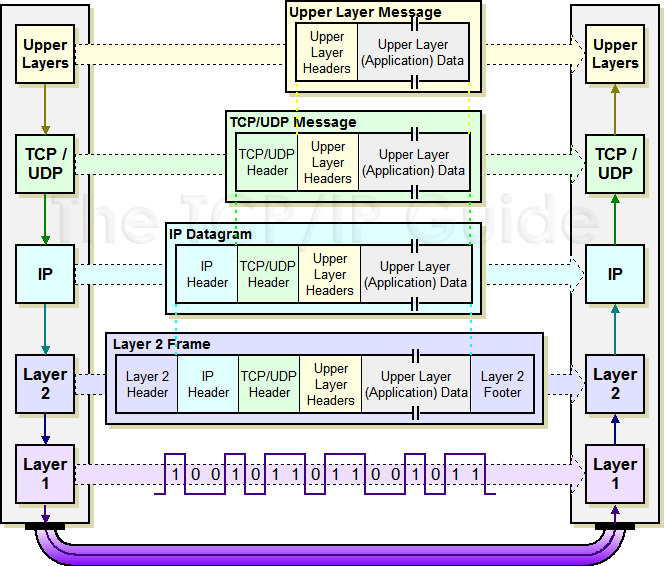
\includegraphics[width=\textwidth]{tcp_encap_2.png}
\caption{分层封装}
\end{figure}

\begin{figure}[H]
\centering
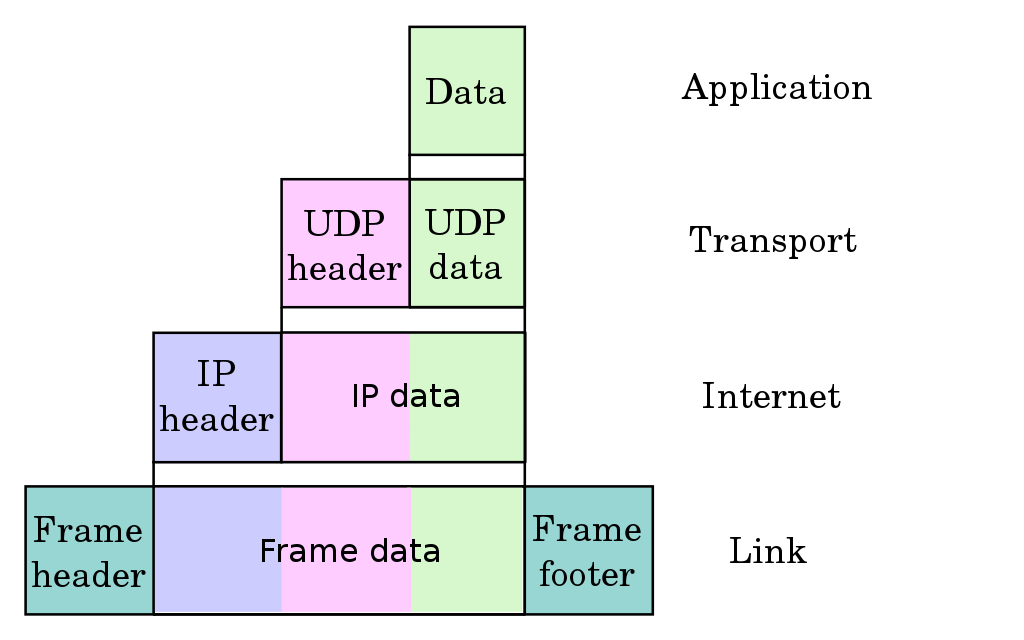
\includegraphics[width=0.4\textwidth]{tcp_encap.png}
\caption{分层封装中的各个帧}
\end{figure}

\begin{figure}[H]
\centering
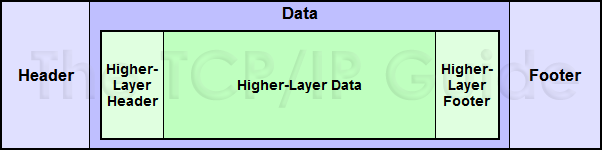
\includegraphics[width=0.8\textwidth]{funformatting.png}
\caption{抽象}
\end{figure}

\section{时延计算}
\subsection{传播时延}
\subsection{信道利用率}

\begin{figure}[H]
\centering
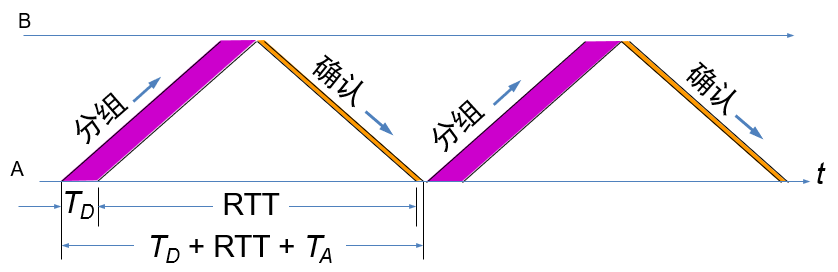
\includegraphics[width=0.8\textwidth]{rtt.png}
\caption{RTT}
\end{figure}
假设A发送分组需要的时间是$T_D$, $T_D$等于分组长度除以数据率。
\begin{equation}
  T_D=\frac{\text{Length (in bit)}}{R_b}
\end{equation}
假定B发送确认分组需要时间$T_A$, 那么A经过时间($T_D+RTT+T_A$)后就可以再发送下一个分组

假定1200km的信道的往返时间RTT\footnote{Round-Trip Time 同一個封包來回時間}=20ms.分组长度是1200bit,发送速率是1Mb/s。若忽略处理时间和$T_A$($T_A$一般远小于$T_D$),计算信道的利用率。
\begin{equation}
  \eta= \frac{T_D}{T_D+RTT+T_A}
\end{equation}
\begin{align*}
  \text{RTT}&=0.02 s\\
  T_D&=\frac{1200}{1\times 10^6}=0.0012 s\\
  \eta&=\frac{T_D}{T_D+\text{RTT}}
\end{align*}


\chapter{Application}
\section{model}
\subsection{P2P}
\subsection{client and server}
\section{HTTP}
TCP 80 port. 

\section{DNS}
UDP 53 port
\begin{itemize}
  \item 根域名服务器
  \item 顶级域名服务器
  \item 本地域名服务器
\end{itemize}

\begin{itemize}
  \item 根域名服务器 (root name server)
  \item 顶级域名 (通用, 国家) www.google.co\texttt{.jp}
  \item 二级域名 www.google\texttt{.co}.jp
  \item 三级域名 www.\texttt{google}.co.jp
  \item 四级域名 \texttt{www}.google.co.jp
\end{itemize}

In the Domain Name System (DNS) hierarchy, a second-level domain (SLD or 2LD) is a domain that is directly below a top-level domain (TLD). For example, in \texttt{example.com}, \texttt{example} is the second-level domain of the \texttt{.com} TLD.
\section{Email}
\begin{itemize}
  \item SMTP\footnote{Simple Mail Transfer Protocol. TCP port 25 } 发邮件
  \item POP3\footnote{Post Office Protocol Version 3. TCP port 110}, IMAP\footnote{Internet Message Access Protocol. TCP port 143 } 收邮件
\end{itemize}
\subsection{SMTP}
\begin{enumerate}
  \item 连接建立
  \item 邮件传送
  \item 连接释放
\end{enumerate}
\section{FTP}
\begin{itemize}
  \item TCP port 21 传请求
  \item TCP port 20 传文件
\end{itemize}

\chapter{Transport}
\section{Interprocess Communication}
\href{https://tldp.org/LDP/tlk/ipc/ipc.html}{Interprocess Communication Mechanisms}

In computer science, inter-process communication or interprocess communication (IPC) refers specifically to the mechanisms an operating system provides to allow the processes to manage shared data. 

\begin{itemize}
  \item Signals
  \item Pipes (named and unnamed)
  \item \textbf{Sockets}
  \item System V IPC
  \subitem Message Queues
  \subitem Semaphore
  \subitem Shared Memory
\end{itemize}
\section{Transmission Control Protocol}
% \begin{itemize}
%   \item 面向连接的协议 Connection-Oriented Protocols: These protocols require that a logical connection be established between two devices before transferring data. This is generally accomplished by following a specific set of rules that specify how a connection should be initiated, negotiated, managed and eventually terminated. Usually one device begins by sending a request to open a connection, and the other responds. They pass control information to determine if and how the connection should be set up. If this is successful, data is sent between the devices. When they are finished, the connection is broken.

%   \item 无连接的协议 Connectionless Protocols: These protocols do not establish a connection between devices. As soon as a device has data to send to another, it just sends it.
% \end{itemize}

\begin{itemize}
  \item 面向连接(虚连接)
  \item 每条TCP连接只能有两个端点, 每条TCP连接只能是点对点的
  \item 可靠交付的服务--无差错, 不丢失, 不重复, 按序到达
  \item 全双工--发送缓存(发送窗口), 接收缓存
  \item 发送字节流
\end{itemize}

\subsection{Segment}
\begin{figure}[H]
\centering
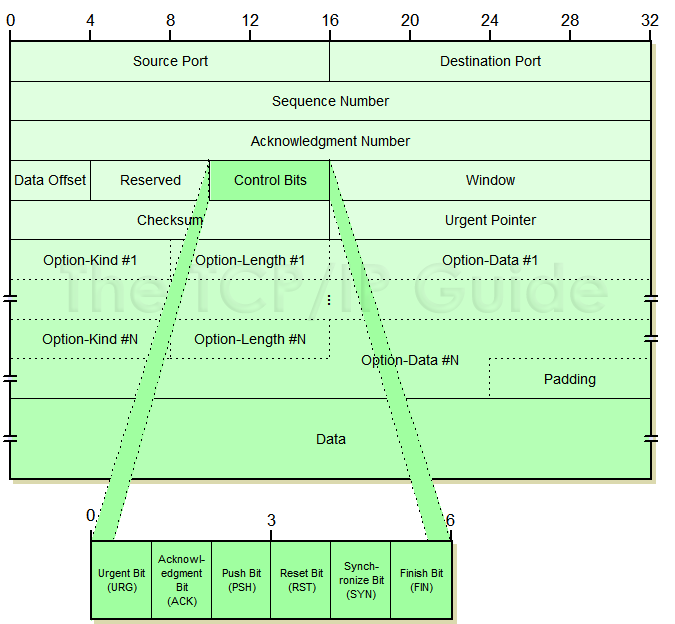
\includegraphics[width=0.8\textwidth]{tcpsegmentformat.png}
\caption{TCP Segment(Message)}
\end{figure}
\paragraph{Data Offset}指示TCP头部的4 Bytes的数目。范围为$5\sim 15$. TCP头部最小为20字节,最大为($15\times4 = 60$)字节

\subsection{Connection establishment}
3 way sync. 三次握手, 前两次不携带数据, 最后一次可以携带用户数据. 
\begin{figure}[H]
\centering
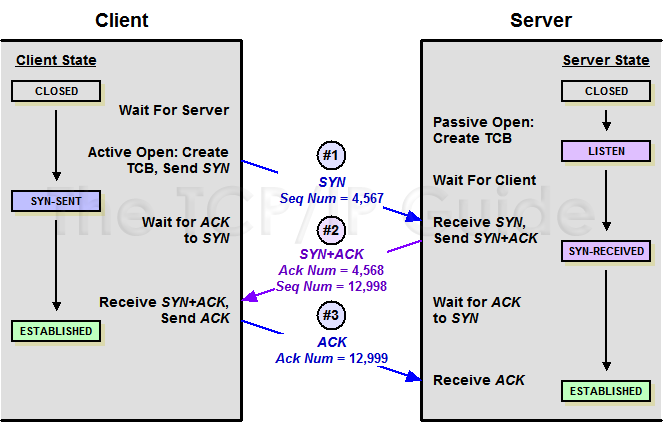
\includegraphics[width=0.6\textwidth]{tcp3waysynch.png}
\caption{TCP Sequence Number Synchronization}
\end{figure}

\begin{figure}[H]
\centering
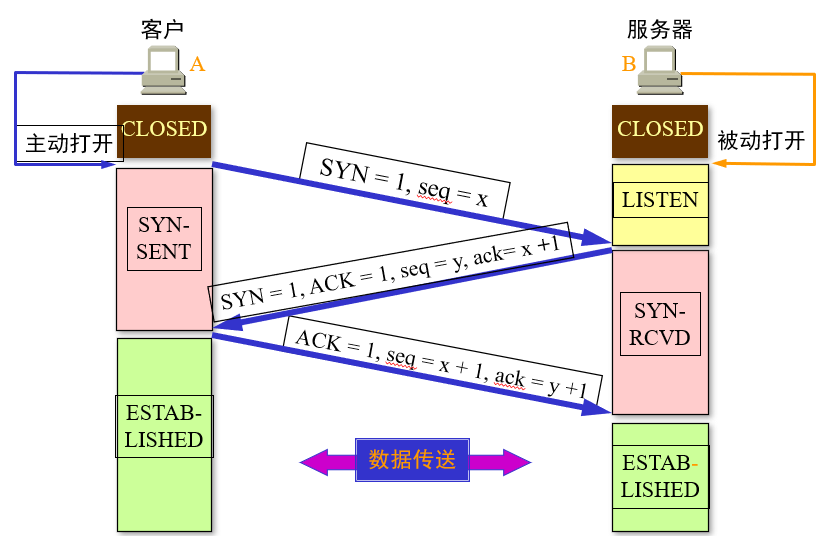
\includegraphics[width=0.6\textwidth]{tcp_est.png}
\caption{TCP 连接建立}
\end{figure}

\begin{figure}[H]
\centering
\begin{verbatim}
      TCP A                                                TCP B

1.  CLOSED                                               LISTEN

2.  SYN-SENT    --> <SEQ=100><CTL=SYN>               --> SYN-RECEIVED

3.  ESTABLISHED <-- <SEQ=300><ACK=101><CTL=SYN,ACK>  <-- SYN-RECEIVED

4.  ESTABLISHED --> <SEQ=101><ACK=301><CTL=ACK>       --> ESTABLISHED

5.  ESTABLISHED --> <SEQ=101><ACK=301><CTL=ACK><DATA> --> ESTABLISHED
\end{verbatim}
\caption{Basic 3-Way Handshake for Connection Synchronization}
\end{figure}

\paragraph{seq}TCP 连接中传送的数据流中的每一个字节都编上一个序号。序号字段的值则指的是本报文段所发送的数据的\textbf{第一个字节的序号}。 对于没有数据的传输,如ACK,虽然它有一个$seq$,但是这次传输在整个data stream中是不占位置的。

\paragraph{ack}是期望收到对方的下一个报文段的数据的第一个字节的序号。 确认号等于N 表明:到序号N-1为止的所有数据都已经正确接收. 
\begin{itemize}
  \item A 的 TCP 向 B 发出连接请求报文段,其首部中的同步位 SYN = 1,并选择序号 $seq = A$\footnote{这个序号随意选择, 被称作initial sequence number(ISN), 但是对方下一次的$ack$必然为其加一. 且自己发送的下一个数据的$seq$也应为其加一},表明传送数据时的第一个数据字节的序号是 A。
\item B 在确认报文段中应使 SYN = 1,使 ACK = 1,其确认号$ack = A + 1$,自己选择的序号 $seq = B$\footnote{同上一脚注}。
\item A 收到此报文段后向 B 给出确认,其 ACK = 1,确认号 $ack = B + 1$。其消息序号为$seq=A+1$
\end{itemize}
\begin{itemize}
  \item SYN
  \subitem The active open is performed by the client sending a SYN to the server. The client sets the segment's sequence number to a random value A.
  \item SYN-ACK
  \subitem In response, the server replies with a SYN-ACK. The acknowledgment number is set to one more than the received sequence number i.e. A+1, and the sequence number that the server chooses for the packet is another random number, B.
  \item ACK
  \subitem Finally, the client sends an ACK back to the server. The sequence number is set to the received acknowledgment value i.e. A+1, and the acknowledgment number is set to one more than the received sequence number i.e. B+1.
\end{itemize}
\subsection{Connection termination}
\begin{figure}[H]
\centering
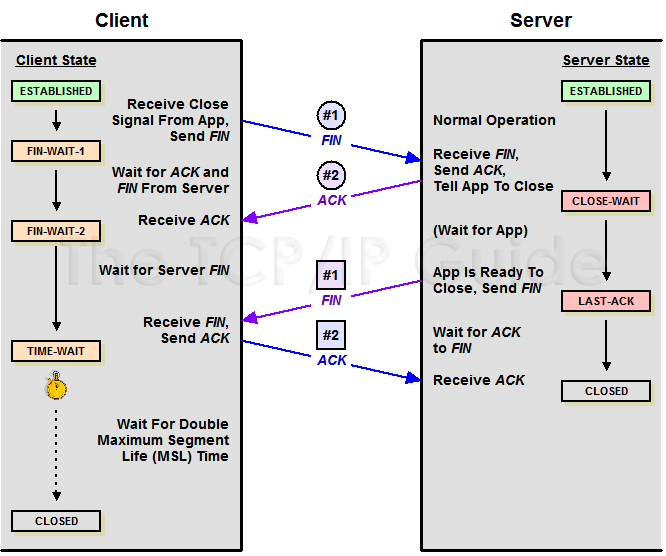
\includegraphics[width=0.6\textwidth]{tcpclose.png}
\caption{TCP Close}
\end{figure}

\begin{figure}[H]
\centering
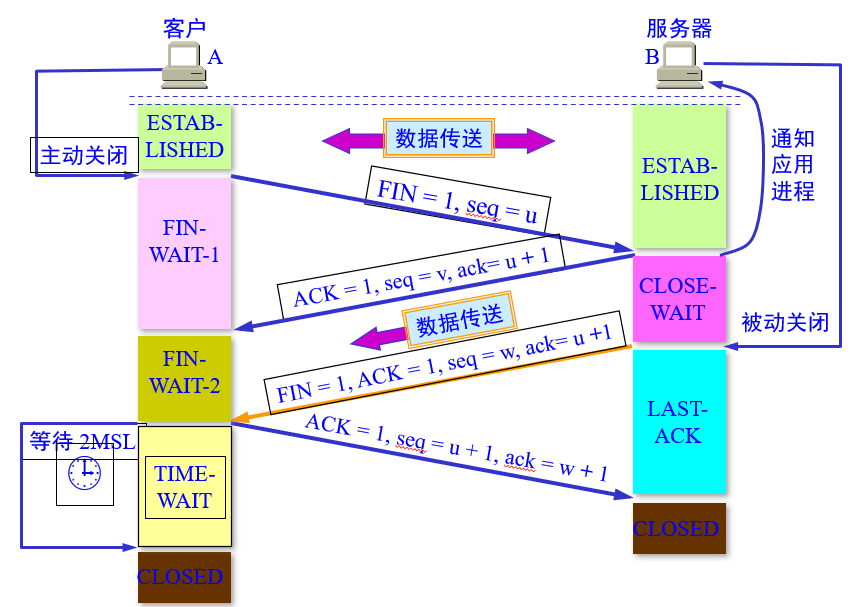
\includegraphics[width=0.6\textwidth]{tcp_close.png}
\caption{TCP Connection Termination}
\end{figure}

\begin{figure}[H]
\centering
\begin{verbatim}
      TCP A                                                TCP B

  1.  ESTABLISHED                                          ESTABLISHED

  2.  (Close)
      FIN-WAIT-1  --> <SEQ=100><ACK=300><CTL=FIN,ACK>  --> CLOSE-WAIT

  3.  FIN-WAIT-2  <-- <SEQ=300><ACK=101><CTL=ACK>      <-- CLOSE-WAIT

  4.                                                       (Close)
      TIME-WAIT   <-- <SEQ=300><ACK=101><CTL=FIN,ACK>  <-- LAST-ACK

  5.  TIME-WAIT   --> <SEQ=101><ACK=301><CTL=ACK>      --> CLOSED

  6.  (2 MSL)
      CLOSED
\end{verbatim}
\caption{Normal Close Sequence}
\end{figure}
称主动连接终止者为A, 目标为B
\begin{itemize}
  \item A 把连接释放报文段首部的 FIN = 1, ACK=1,其序号$seq = u$\footnote{承接上一个自己发的Segment的 seq}, 确认号承接上一个B发送的消息的$seq$, \footnote{假设上一个B发送消息的$seq$为$v-1$}$ack=v$,等待 B 的确认。
  \item B 发出确认,确认号$ack = u +1$\footnote{期望A回复带有ACK的报文, 但是在B发出\textbf{FIN-ACK}之前A是不会回复的}, $seq = v$。
  \subitem TCP 服务器进程通知高层应用进程。从 A 到 B 这个方向的连接就释放了
  \subitem TCP 连接处于半关闭状态。B 若发送数据,A 仍要接收。
  \item B 若发送数据,A 仍要接收。
  \item B此时作为连接终止者, FIN = 1, ACK = 1, $seq = w$\footnote{如果上一条数据是B的\textbf{ACK}那么这一条的$seq$仍然为$v$. 因为\textbf{ACK}不会增加自身的$seq$号, 但是\textbf{FIN}会}, $ack= u +1$
  \subitem 期望A回复带有ACK的报文
  \item A发送最后一条\textbf{ACK}即 ACK = 1, $seq = u + 1$, $ack = w + 1$
\end{itemize}


等待计时器设置的2MSL(maximum segment life)后连接彻底关闭. 
\begin{itemize}
  \item 为了保证终止发起者发送的最后一个 ACK 报文段能够到达目标。
  \item 防止老的重复分组在本次连接结束之前再次建立新连接。
\end{itemize}
\section{TCP Reliability and Flow Control Features}
% The Transmission Control Protocol uses a variant of Go-Back-N ARQ to ensure reliable transmission of data over the Internet Protocol, which does not provide guaranteed delivery of packets; with Selective Acknowledgement (SACK) extension, it may also use Selective Repeat ARQ.


% 对发送方而言有以下情况
% \begin{enumerate}
%  \item Bytes Sent And Acknowledged
%  \item Bytes Sent But Not Yet Acknowledged
%  \item Bytes Not Yet Sent For Which Recipient Is Ready
%  \item Bytes Not Yet Sent For Which Recipient Is Not Ready
% \end{enumerate}
% 对接收方而言

% \begin{enumerate}
%   \item  收到且已经ACK. 
%   \item  还没收到的Bytes, 但是大概要发过来
%   \item  还没收到的Bytes, 但是可能不会发过来 (那么快)
% \end{enumerate}


\subsection{Selective ACK (SACK)}
Given the maximum size of the TCP option field (40 bytes), an ACK packet can carry at most 4 Sack blocks. 

\subsection{Flow Control}
\subsubsection{Receive Window}
\label{sec:tcp_rwnd}
传输窗口: 在\textbf{ACK} 收到之前最多能发送的数据
\subsubsection{Send Window}
\label{sec:tcp_swnd}
发送方的发送窗口的上限值应当取为接收方窗口 rwnd(见\ref{sec:tcp_rwnd}) 和拥塞窗口 cwnd(见\ref{sec:tcp_cwnd}) 这两个变量中较小的一个

\paragraph{控制TCP报文段的发送时机}
\begin{enumerate}
  \item TCP维持一个变量,它等于最大报文段长度 MSS\footnote{ 最大报文段 (Maximum Segment Size) MSS针对的是OSI模型里第四层传输层的TCP协议。}。只要缓存中存放的数据达到 MSS 字节时,就组装成一个 TCP 报文段发送出去。
  \item 由发送方的应用进程指明要求发送报文段,即 TCP 支持的推送(push)操作。
  \item 发送方的一个计时器期限到了,这时就把当前已有的缓存数据装入报文段(但长度不能超过 MSS)发送出去。
\end{enumerate}

\begin{equation}
  \text{发送窗口的上限值} = \min [\text{rwnd}, \text{cwnd}]
\end{equation}

\begin{itemize}
  \item 当 rwnd < cwnd 时,是接收方的接收能力限制发送窗口的最大值。
  \item 当 cwnd < rwnd 时,则是网络的拥塞限制发送窗口的最大值。 
\end{itemize}
滑动窗口 Sliding Window. 让发送方发慢点. 

在接收方设置的确认报文段的\textbf{窗口字段}来将接收窗口通知给发送方. 

接收窗口, 拥塞窗口\footnote{发送方根据自己估算的网络拥塞程度而设置的窗口值, 反映网络当前容量}. 
\subsection{Congestion Control}
基于丢包反馈属于被动式机制,根源在于这些拥塞控制算法依据是否出现丢包事件来判断网络拥塞做减窗调整. 
\paragraph{主要方式}
\begin{itemize}
  \item 慢开始
  \item 加法增大 (拥塞避免)
  \item 乘法减小
  \item 收到三个重复的确认, 执行快重传
  \item 快恢复 (TCP Reno版本\footnote{算法太多啦 看看 BBR}) 
\end{itemize}

% \begin{itemize}
%   \item \href{https://zh.wikipedia.org/wiki/TCP%E6%8B%A5%E5%A1%9E%E6%8E%A7%E5%88%B6}{TCP 拥塞控制}
%   \item \href{https://en.wikipedia.org/wiki/TCP_congestion_control}{TCP Congestion Control}
% \end{itemize}
\subsubsection{Congestion Window/慢开始}
\label{sec:tcp_cwnd}
发送方维持一个叫做拥塞窗口 cwnd (congestion window)的状态变量。拥塞窗口的大小取决于网络的拥塞程度,并且动态地在变化。发送方让自己的发送窗口等于拥塞窗口。

使用慢开始算法后,每经过一个传输轮次,拥塞窗口 cwnd 就加倍。 一个传输轮次所经历的时间就是往返时间 RTT

\paragraph{ssthresh}拥塞窗口cwnd增长过大引起网络拥塞,还需要设置一个慢开始门限ssthresh状态变量。

\subsubsection{AIMD}
乘法减小, 加法增大 (AIMD\footnote{additive-increase/multiplicative-decrease}线性增乘性减)
\paragraph{MD}只要出现一次超时(即出现一次网络拥塞),就把慢开始门限值 ssthresh 设置为当前的拥塞窗口值的一半
\paragraph{AI}是指执行拥塞避免算法后,在收到对所有报文段的确认后(即经过一个往返时间),就把拥塞窗口 cwnd增加一个 MSS 大小,使拥塞窗口缓慢增大
\begin{figure}[H]
\centering
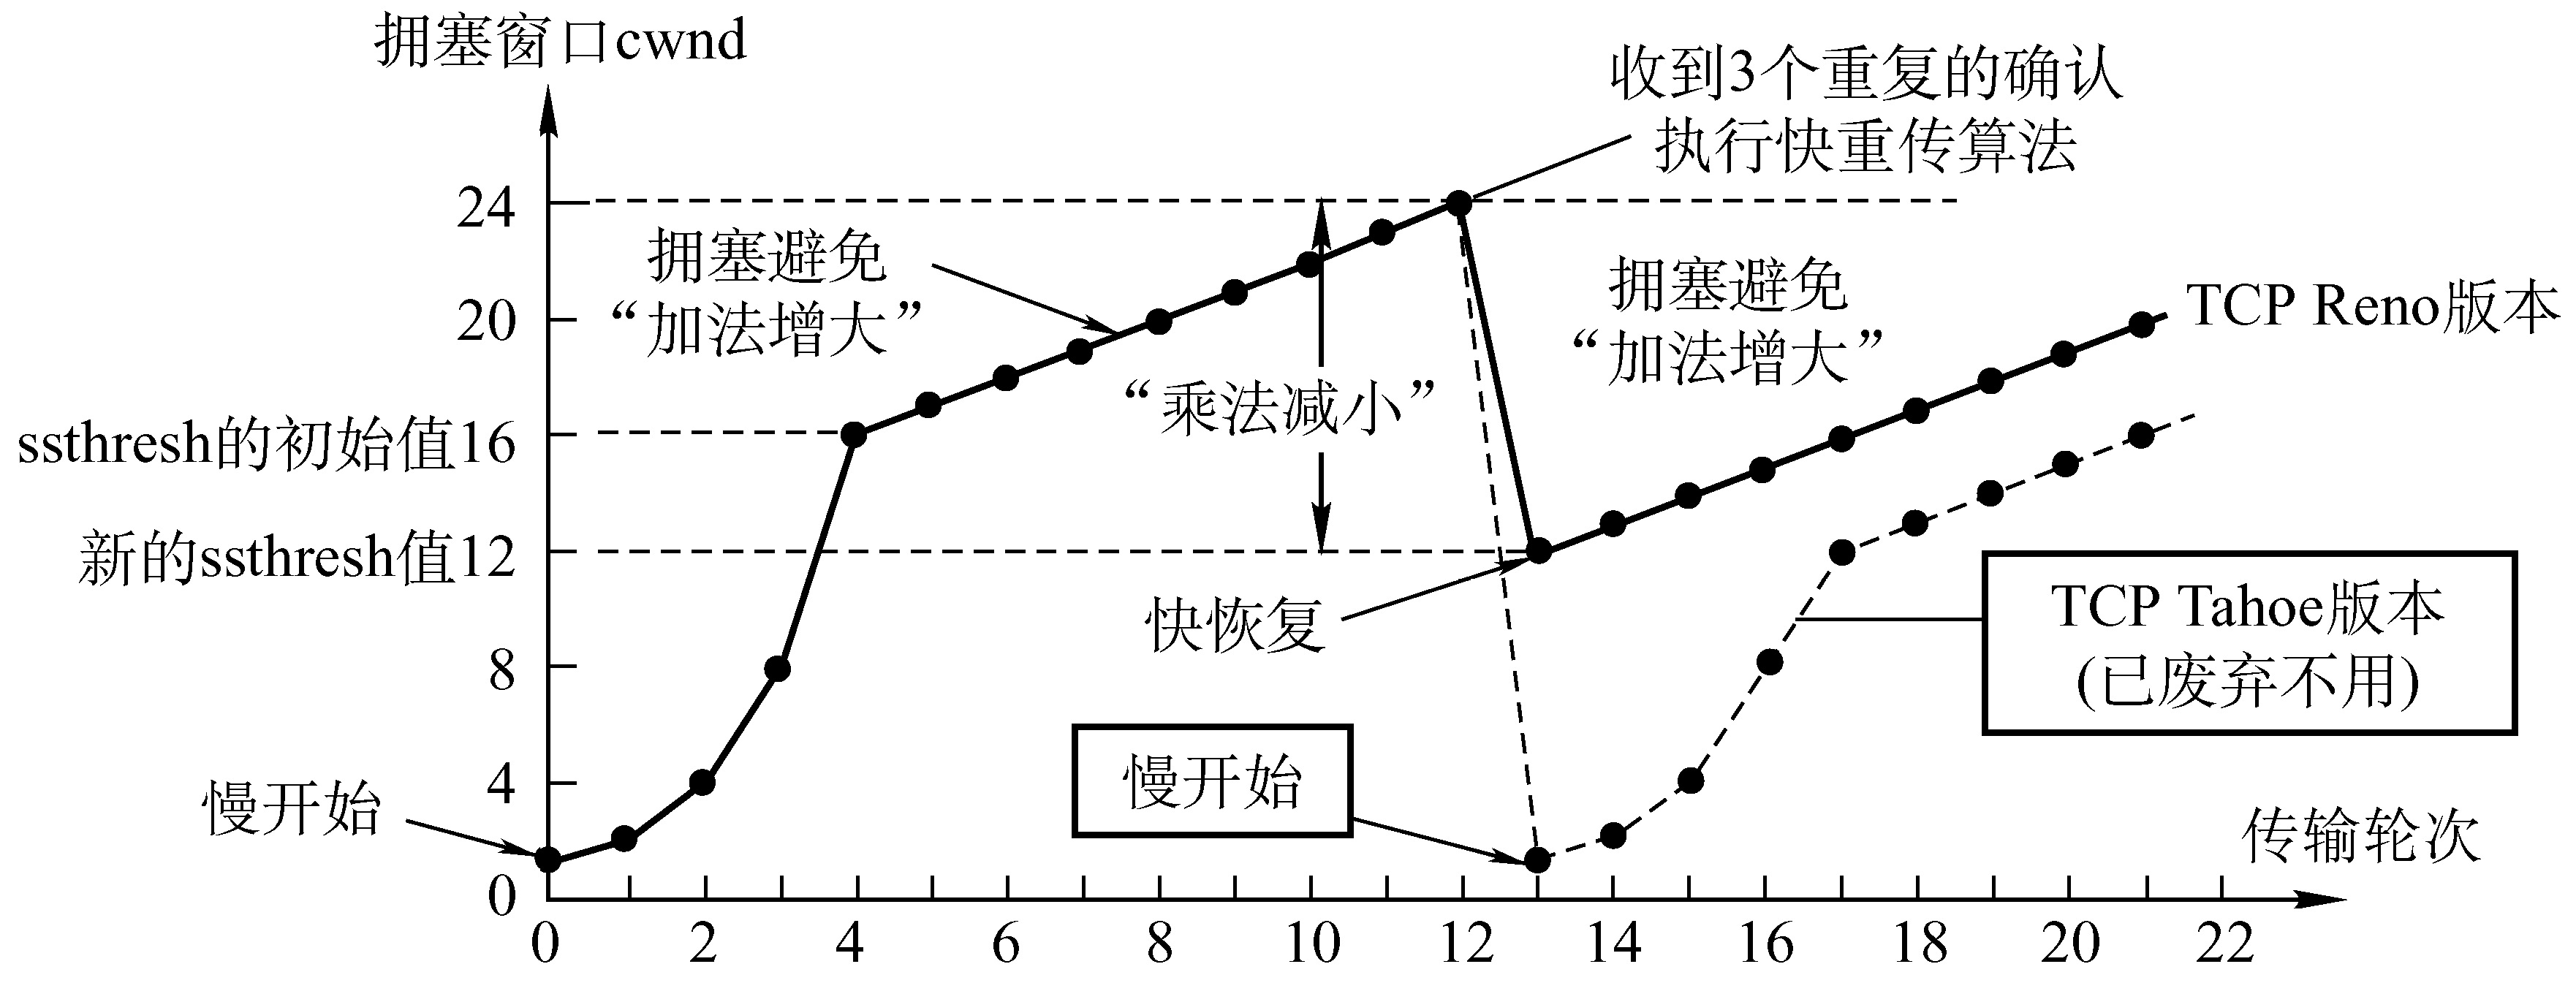
\includegraphics[width=0.6\textwidth]{tcp_traffic.png}
\caption{AIMD和快重传}
\end{figure}


\subsubsection{拥塞控制和流量控制的区别与联系}
拥塞控制: 防止过多的数据注入到网络中,这样可以使网络中的路由器或链路不致过载。所要做的都有一个前提,就是网络能够承受现有的网络负荷。
\begin{itemize}
  \item 拥塞控制是一个全局性的过程,涉及到所有的主机、所有的路由器,以及与降低网络传输性能有关的所有因素。 
  \item 流量控制往往指在给定的发送端和接收端之间的点对点通信量的控制,是个端到端的问题。 
  \item 流量控制所要做的就是抑制发送端发送数据的速率,以便使接收端来得及接收。 
\end{itemize}


\section{User Datagram Protocol}
\begin{figure}[H]
\centering
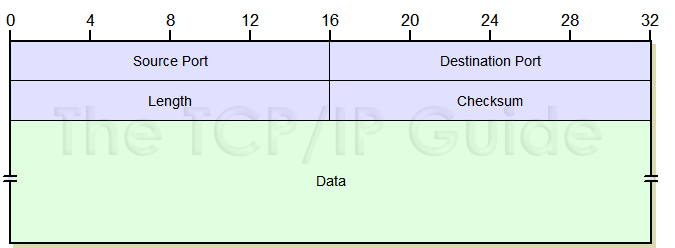
\includegraphics[width=0.8\textwidth]{udpformat.png}
\caption{UDP Message}
\end{figure}
\subsection{Checksum}
\href{https://en.wikipedia.org/wiki/User_Datagram_Protocol#Checksum_computation}{Checksum Computation}

Checksum is the 16-bit one's complement of the \textbf{one's complement sum of a pseudo header of information from the IP header}, the UDP header, and the data,  padded  with zero octets  at the end (if  necessary)  to  make  a multiple of two octets.

When UDP runs over IPv6, the checksum is mandatory. 

\begin{figure}[H]
\centering
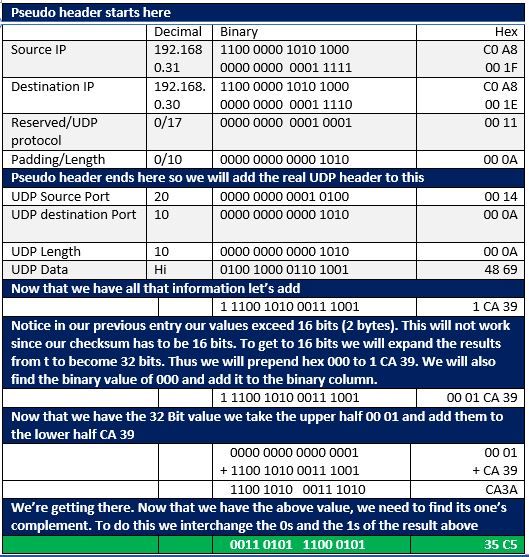
\includegraphics[width=0.6\textwidth]{udp_checksum.jpg}
\caption{检查和计算}
\end{figure}
\begin{itemize}
  \item 检查和必定是固定的, 在这里是每16 bit为一个单位. 
  \item 把要发的数据按照 16 bit 为单位分割
  \item 正常加, 带进位的, 不是模二加. 可以用十六进制来做, 头不会那么晕. 
  \item 如果超出了 16 bit 不用怕, 给它扩展到 32 bit, 等到最后再把高 16 bit 加起来. 
  \item 记得最后要取one's complement, 即每位取反. 
\end{itemize}

\begin{figure}[H]
\centering
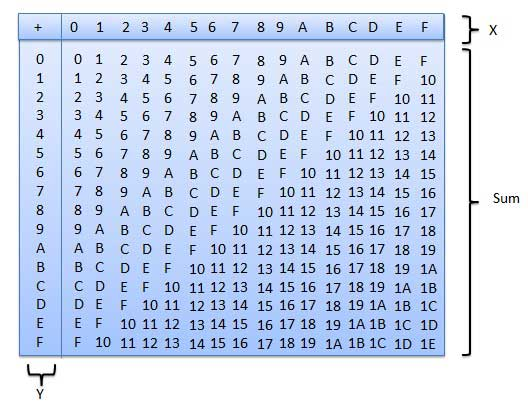
\includegraphics[width=0.6\textwidth]{hex_add_table.jpg}
\caption{十六进制加法表}
\end{figure}
或者如果遇到进位, 就把它拆成 16 (进高位) + 余数 (保留低位). 记住A是10, 才是11, F是15而非16. 

B+B=11+11=22=16+6=16


\chapter{Network}
\begin{itemize}
  \item 灵活的
  \item 无连接的
  \item 尽最大努力交付的数据报服务
\end{itemize}

\begin{itemize}
  \item 分组间的定时不能被保证;
  \item 分组的接收顺序与发送顺序不一定相同;
  \item 传送的分组不能保证最终交付,即网络可能未向目的地交付分组。
\end{itemize}


\section{IPv4 Datagram}

\begin{figure}[H]
\centering
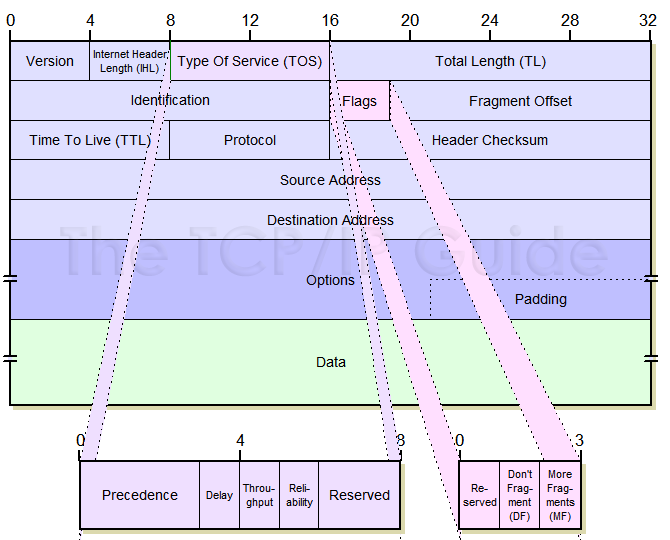
\includegraphics[width=0.8\textwidth]{ipformat.png}
\caption{IP Datagram}
\end{figure}
\begin{figure}[H]
\centering
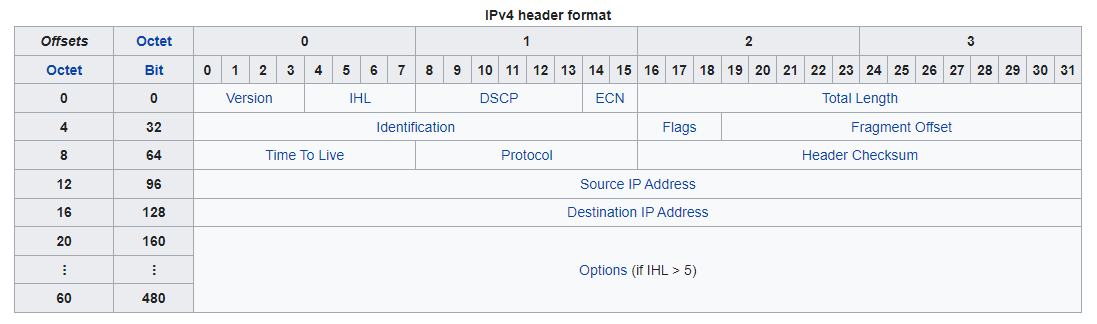
\includegraphics[width=\textwidth]{ip_header.png}
\caption{IP Header}
\end{figure}
\begin{itemize}
  \item Version
  \subitem IPv4中总是等于4
  \item Internet Header Length (4 bits)
  \subitem 这玩意是标明IPv4头部长度的, 不是标明Ethernet Frame的长度的. 
  \subitem TCP头部. 跟IP头长度一样,20~60 Bytes
  \subitem The IPv4 header is variable in size due to the optional 14th field (options). The IHL field contains the size of the IPv4 header, it has \emph{4 bits that specify the number of 32-bit(4 Bytes) words in the header.} \textbf{The minimum value for this field is 5, which indicates a length of 5 × 32 bits = 160 bits = 20 bytes.} As a 4-bit field, the maximum value is 15, this means that the maximum size of the IPv4 header is 15 × 32 bits = 480 bits = 60 bytes.
  \subitem IPv4 头部长度等于 $\text{IHL}\times 4$ Bytes. IHL最小值为5, 最大值为15 (4 bit即$2^4-1$)
  \item Differentiated Services Code Point 
  \subitem Type Of Services (TOS) Real-time data streaming makes use of the DSCP field. An example is Voice over IP (VoIP), which is used for interactive voice services.
  \item Explicit Congestion Notification 
  \subitem 可选, 表示网络堵塞. 
  \item Total Length
  \subitem 首部加上数据的长度. The minimum size is 20 bytes (header without data) and the maximum is 65,535\footnote{$2^{16}$} bytes. 
  \subitem All hosts are required to be able to reassemble datagrams of size up to 576 bytes, but most modern hosts handle much larger packets. 
  \subitem Links may impose further restrictions on the packet size, in which case datagrams must be fragmented. 
  \subitem 对于以太网来说, 数据部分超过 1500 Bytes 就会被分片. 所以通常 IP datagram/packet 的长度不会超过 1500 Bytes. 
  \item Identification
  \subitem This field is an identification field and is primarily used for uniquely identifying the group of fragments of a single IP datagram. \textbf{同一数据报的分片使用同一标识}. 
  \item Flag
  \item Fragment Offset
  \subitem 见 IP 数据报的切割 \ref{sec:ip_fragment} 一节
  \item Time To Live
  \subitem 存活跳数(hop), 过一个路由就减一. 8 bit即$2^8-1=255$. 
  \item Protocol
  \subitem RFC 790 中定义的协议. 见\href{https://en.wikipedia.org/wiki/List_of_IP_protocol_numbers}{List of IP protocol numbers}. 其中定义了ICMP (0x01), IGMP (0x02), TCP (0x06), UDP (0x17)
  \item Header Checksum
  \subitem 只检验首部
  \subitem \href{https://en.wikipedia.org/wiki/IPv4_header_checksum}{IPv4 header checksum} When a packet arrives at a router, the router calculates the checksum of the header and compares it to the checksum field. If the values do not match, the router discards the packet.
  \item Source
  \item Destination
  \item Options
  \subitem The options field is not often used. Note that the value in the IHL field must include enough extra 32-bit words to hold all the options (plus any padding needed to ensure that the header contains an integer number of 32-bit words). 
  \subitem The list of options may be terminated with an EOL (End of Options List, 0x00) option; this is only necessary if the end of the options would not otherwise coincide with the end of the header. 
  \item Data 
\end{itemize}

把分组(IP datagram)通过路由选择与转发从源端传送到目的端. 为分组交换网上的不同主机提供通信服务. 

\subsection{IP datagram fragment}
\begin{figure}[H]
\centering
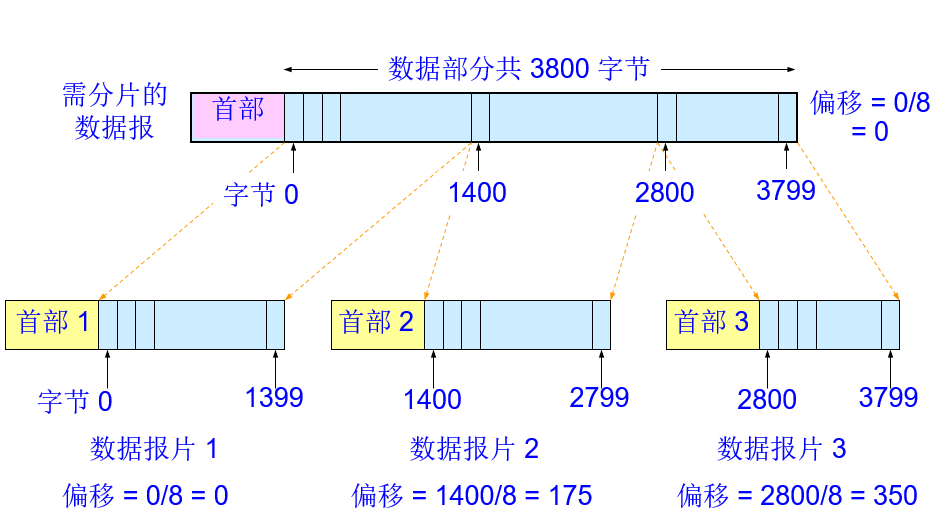
\includegraphics[width=0.8\textwidth]{ip_frag.png}
\caption{IP 分段}
\end{figure}

\begin{figure}[H]
\centering
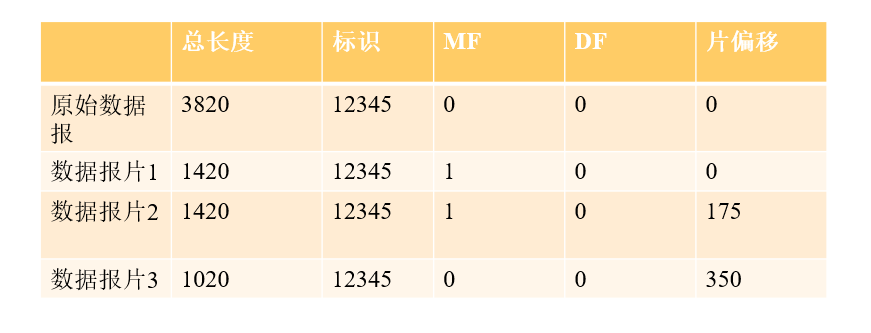
\includegraphics[width=\textwidth]{ip_frag_tab.png}
\caption{IP 分段表格}
\end{figure}

\begin{itemize}
  \item Identities 对于同一数据报的分段值应该一样
  \item 偏移中的值是以 8 Bytes 为单位
\end{itemize}

\label{sec:ip_fragment}

\section{IPv6 Datagram}
\begin{figure}[H]
\centering
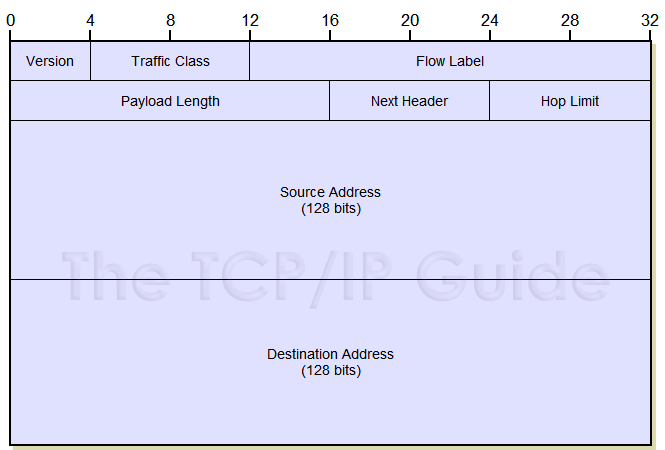
\includegraphics[width=0.8\textwidth]{ipv6format.png}
\caption{IPv6}
\end{figure}
\begin{itemize}
  \item 首部固定为 40 Byte, 不再有可变选项
  \item 首部校验和(Header Checksum)消失
  \item IPv6 没有 Fragmentation (分片)
  \item 使用 CDIR 标识, 只能以 4 bit 为单位划分子网. 
  \item IPv6本地链路地址以fe80::/10开头,通常由系统自动为每个网络设备生成。
\end{itemize}
\subsection{IPv6 EUI-64}
EUI-64 (Extended Unique Identifier) is a method we can use to automatically configure IPv6 host addresses. An IPv6 device will use the MAC address of its interface to generate a unique 64-bit interface ID. 

\begin{figure}[H]
\centering
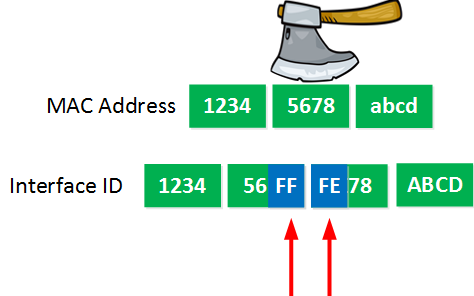
\includegraphics[width=0.5\textwidth]{ipv6_eui.png}
\caption{IPv6 EUI64}
\end{figure}

\begin{enumerate}
  \item MAC地址的前 3 Bytes, 加 FF, 加FE, 后 3 Bytes, 得到EUI64
  \item 再将EUI-64地址的\textbf{第一字节第 7 bit为反转},形成IPv6地址的接口ID
  \item 从网关得到IPv6地址前缀,64bit的地址前缀加上通过EUI-64生成的地址后缀
  \item 若生成的是链路本地地址(Link-Local Address)则加上FE80的前缀即可
\end{enumerate}



\subsection{Abbreviation}
\begin{itemize}
  \item The IPv6 addressing architecture allows you use the two-colon (::) notation to represent contiguous 16-bit fields of zeros. 
  \item Other fields of zeros can be represented as a single 0.
  \item You can also omit any leading zeros in a field, such as changing 0db8 to db8.
\end{itemize}

\section{IP Class}
\subsection{Binary Conversion}
取一个数, 放最右边, 除以2, 余数写下边作为LSB\footnote{Least Significant Bit}. 商写数的左边. 递归, 直到商为0. 最后得到的位是MSB\footnote{Most Significant Bit}

还有一种方法. 对于位数确定(范围确定的)数, 如以下说的 8 bit (0$\sim$255) 的情况. 可以直接列表, 如表\ref{tab:bin_add}和\ref{tab:bin_add_2}. 注意在这种算法中是由\textbf{MSB}到\textbf{LSB}推导的, 与上一种不同. 
\begin{itemize}
  \item 0+128=128<244 上 1
  \item 128+64=192<244 上 1
  \item 192+32=224<244 上 1
  \item 224+16=240<244 上 1
  \item 240+8=248>244 上 0 
  \item 240+4=244=244 上 1 结束
  \item 尾部补0即可
\end{itemize}

\subsection{Class}
A classful network is a network addressing architecture used in the Internet from 1981 until the introduction of Classless Inter-Domain Routing in 1993. 

 In the olden days, there were Class A, B and C networks. These could only be divided up into equal parts, so VLSM, or Variable Length Subnet Masks , were introduced. The old Class C was a /24, B was a /16, and A was a /8. That’s all you need to know about Classes. They don’t exist anymore.

\begin{itemize}
  \item Class A networks use a default subnet mask of 255.0.0.0 and have 0-127 as their first octet. The address 10.52.36.11 is a class A address. Its first octet is 10, which is between 1 and 126, inclusive.
  \item Class B networks use a default subnet mask of 255.255.0.0 and have 128-191 as their first octet. The address 172.16.52.63 is a class B address. Its first octet is 172, which is between 128 and 191, inclusive.
  \item Class C networks use a default subnet mask of 255.255.255.0 and have 192-223 as their first octet. The address 192.168.123.132 is a class C address. Its first octet is 192, which is between 192 and 223, inclusive.
\end{itemize}

% Table generated by Excel2LaTeX from sheet 'Sheet3'
% Table generated by Excel2LaTeX from sheet 'Sheet3'
{
  \tiny
\begin{table}[htbp]
  \centering
    \begin{tabular}{ccccccc}
      \hline
    Class & Leading bits & CIDR & Number of networks & Addr/network & Start & End \\
    \hline
    Class A & 0     & /8    & $2^7-2$ & $2^{24}-2$ & 0.0.0.0 & 127.255.255.255 \\
    Class B & 10    & /16   & $2^{14}-1$ & $2^{16}-2$ & 128.0.0.0 & 191.255.255.255 \\
    Class C & 110   & /24   & $2^{21}-1$ & $2^8-2$ & 192.0.0.0 & 223.255.255.255 \\
    Class D (multicast) & 1110  & N/A & N/A & N/A & 224.0.0.0 & 239.255.255.255 \\
    Class E (reserved) & 1111  & N/A & N/A & N/A & 240.0.0.0 & 255.255.255.255 \\
    \hline
    \end{tabular}%
  \label{tab:ip_class}%
  \caption{IP 分类}
\end{table}%
}
{\tiny
% Table generated by Excel2LaTeX from sheet 'Sheet1'
\begin{table}[htbp]
  \centering
    \begin{tabular}{cc}
      \hline
    Binary & Decimal \\
    \hline
    0000 0001 & 1 \\
    0000 0010 & 2 \\
    0000 0100 & 4 \\
    0000 1000 & 8 \\
    0001 0000 & 16 \\
    0010 0000 & 32 \\
    0100 0000 & 64 \\
    1000 0000 & 128 \\
    1100 0000 & 128+64=192 \\
    1110 0000 & 192+32=224 \\
    1111 0000 & 224+16=240 \\
    1111 1000 & 248 \\
    1111 1100 & 252 \\
    1111 1110 & 254 \\
    1111 1111 & 255 \\
    \hline
    \end{tabular}%
  \caption{二进制表}
  \label{tab:binary_table}%
\end{table}%

}
% Table generated by Excel2LaTeX from sheet 'Sheet2'
\begin{table}[htbp]
  \centering
    \begin{tabular}{|l|rrrrrrrrr|}
    Bit   & 7     & 6     & 5     & 4     & 3     & 2     & 1     & 0     & Sum \\
    Decimal & 128   & 64    & 32    & 16    & 8     & 4     & 2     & 1     & 255 \\
    Binary & 1     & 1     & 1     & 1     & 0     & 1     & 0     & 0     & 244 \\
    \end{tabular}%
  \caption{二进制加法表}
  \label{tab:bin_add_2}%
\end{table}%

% Table generated by Excel2LaTeX from sheet 'Sheet2'
\begin{table}[htbp]
  \centering
    \begin{tabular}{ccccc}
      \hline
    Accumulator & Summand & Sum   & Is Target & Binary \\
    \hline
    0     & 128   & 128   & <     & 1 \\
    128   & 64    & 192   & <     & 1 \\
    192   & 32    & 224   & <     & 1 \\
    224   & 16    & 240   & <     & 1 \\
    240   & 8     & 248   & >     & 0 \\
    240   & 4     & 244   & =     & 1 \\
    -     & -     & -     & -     & 0 \\
    -     & -     & -     & -     & 0 \\
    \hline
    \end{tabular}%
  \caption{加法流程}
  \label{tab:bin_add}
\end{table}%

网络号/主机号一般来说全1/全0不合法. 
\begin{itemize}
  \item 对于 A 类来说, 网络号全1即, 127.x.x.x 为回环 (loopback) 地址. 不合法. 
  \item 对于 A, B, C类, 网络号全 0 不合法. 本网范围内表示主机, 路由表内表示默认路由
  \item 对于主机号, 全0, 全1均不合法. 
  \item 主机号全0表示网络地址, 代表一个网络
  \item 主机号全1表示广播. 
\end{itemize}
\subsection{私有地址}
私有地址亦不合法. 路由器对目的地址时私有IP地址的数据报一律不进行转发. 
% Table generated by Excel2LaTeX from sheet 'Sheet3'
\begin{table}[htbp]
  \centering
    \begin{tabular}{cccc}
      \hline
    IP address range & Number of addr & Largest CIDR block & Classful description \\
    \hline
    10.0.0.0 $\sim$ 10.255.255.255 & 16777216 & 10.0.0.0/8  & single class A network \\
    172.16.0.0 $\sim$ 172.31.255.255 & 1048576 & 172.16.0.0/12  & 16 contiguous class B networks \\
    192.168.0.0 $\sim$ 192.168.255.255 & 65536 & 192.168.0.0/16  & 256 contiguous class C networks \\
    \hline
    \end{tabular}%
  \caption{私有IP地址范围}
  \label{tab:ip_private}%
\end{table}%
地址数量
\begin{itemize}
  \item Class A $1 \times (2^{24}-2)=16777214$
  \item Class B $16\times (2^{16}-2)=1048544$
  \item Class C $256\times (2^{8}-2) =65024$
\end{itemize}

\section{Subnetting}
\href{https://en.wikipedia.org/wiki/Subnetwork}{Subnetwork}: A subnetwork or subnet is a logical subdivision of an IP network.
\subsection{子网划分}
划分子网的时候全0和全1的子网号是无效的
\begin{figure}[H]
\centering
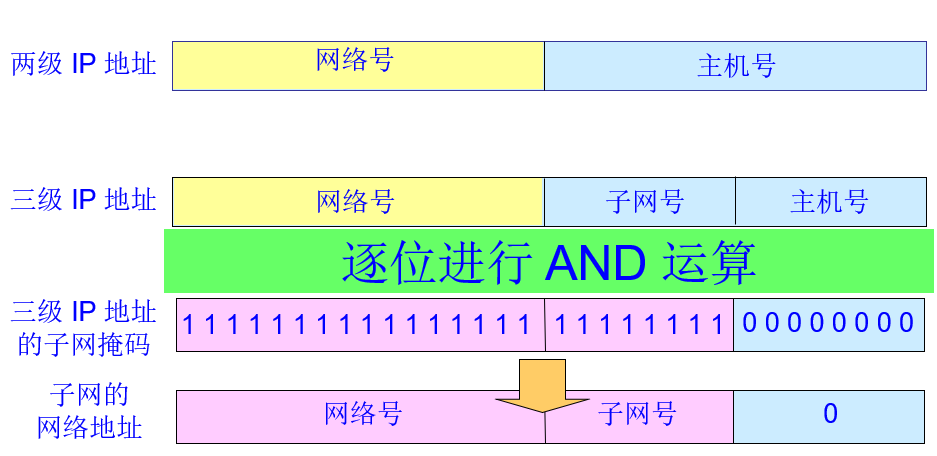
\includegraphics[width=0.6\textwidth]{ip_subnet_mask.png}
\caption{已知 IP 地址是 141.14.72.24,子网掩码是 255.255.192.0; 试求网络地址 }
\end{figure}

\begin{figure}[H]
\centering
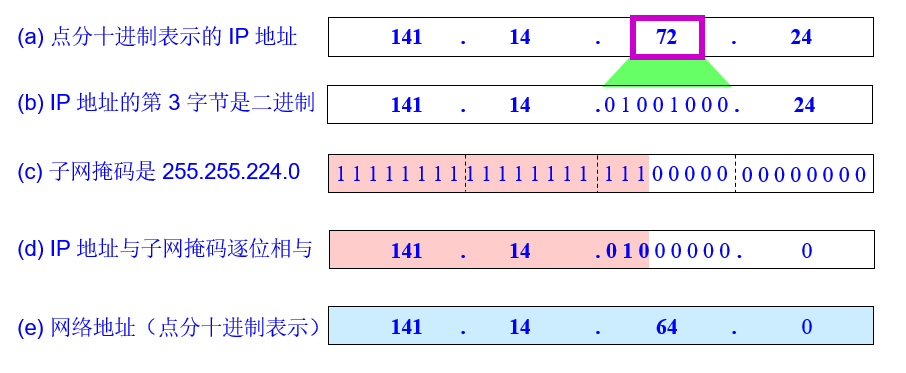
\includegraphics[width=0.6\textwidth]{ip_submask_exp_2.png}
\caption{已知 IP 地址是 141.14.72.24若子网掩码改为255.255.224.0; 试求网络地址}
\end{figure}
不同的子网掩码得出相同的网络地址。(但是仍然是不同的网络)

\subsection{例子}

In order to subnet a network, extend the natural mask with some of the bits from the host ID portion of the address in order to create a subnetwork ID. For example, given a Class C network of 204.17.5.0 which has a natural mask of 255.255.255.0, you can create subnets in this manner:
\begin{verbatim}
  204.17.5.0 -      11001100.00010001.00000101.00000000
  255.255.255.224 - 11111111.11111111.11111111.11100000
                    --------------------------|sub|----
\end{verbatim}
By extending the mask to be 255.255.255.224, you have taken three bits (indicated by "sub") from the original host portion of the address and used them to make subnets. With these three bits, it is possible to create eight subnets. With the remaining five host ID bits, each subnet can have up to 32 host addresses, 30 of which can actually be assigned to a device since host ids of all zeros or all ones are not allowed (it is very important to remember this). So, with this in mind, these subnets have been created.
\begin{verbatim}
204.17.5.0 255.255.255.224     host address range 1 to 30 //not valid? 
204.17.5.32 255.255.255.224    host address range 33 to 62
204.17.5.64 255.255.255.224    host address range 65 to 94
204.17.5.96 255.255.255.224    host address range 97 to 126
204.17.5.128 255.255.255.224   host address range 129 to 158
204.17.5.160 255.255.255.224   host address range 161 to 190
204.17.5.192 255.255.255.224   host address range 193 to 222
204.17.5.224 255.255.255.224   host address range 225 to 254 //not valid? 
\end{verbatim}

\paragraph{Example} Using a subnet mask of 255.255.255.192, your 192.168.123.0 network then becomes the four networks 192.168.123.0, 192.168.123.64, 192.168.123.128 and 192.168.123.192. These four networks would have as valid host addresses


Remember, again, that binary host addresses with all ones or all zeros are invalid, so you can't use addresses with the last octet of 0, 63, 64, 127, 128, 191, 192, or 255.

You can see how it works by looking at two host addresses, 192.168.123.71 and 192.168.123.133. If you used the default Class C subnet mask of 255.255.255.0, both addresses are on the 192.168.123.0 network. However, if you use the subnet mask of 255.255.255.192, they are on different networks; 192.168.123.71 is on the 192.168.123.64 network, 192.168.123.133 is on the 192.168.123.128 network.

\section{Classless Inter-Domain Routing}
\begin{itemize}
  \item CIDR 消除了传统的 A 类、B 类和 C 类地址以及划分子网的概念,因而可以更加有效地分配 IPv4 的地址空间。
  \item CIDR使用各种长度的“网络前缀”(network-prefix)来代替分类地址中的网络号和子网号。
  \item IP地址从三级编址(使用子网掩码)又回到了两级编址。  
  \item CIDR 虽然不使用子网了,但仍然使用“掩码”这一名词(但不叫子网掩码)。
\end{itemize}


There are two ways to denote these masks. First, since you use three bits more than the "natural" Class C mask, you can denote these addresses as having a 3-bit subnet mask. Or, secondly, the mask of 255.255.255.224 can also be denoted as /27 as there are 27 bits that are set in the mask. This second method is used with CIDR. With this method, one of these networks can be described with the notation prefix/length. For example, 204.17.5.32/27 denotes the network 204.17.5.32 255.255.255.224. When appropriate, the prefix/length notation is used to denote the mask throughout the rest of this document.

\section{Network Address Translation}
\section{Protocols}
\subsection{Internet Control Message Protocol}
\begin{itemize}
  \item ICMP 差错报告报文
  \item ICMP 查询报文
\end{itemize}
\begin{figure}[H]
\centering
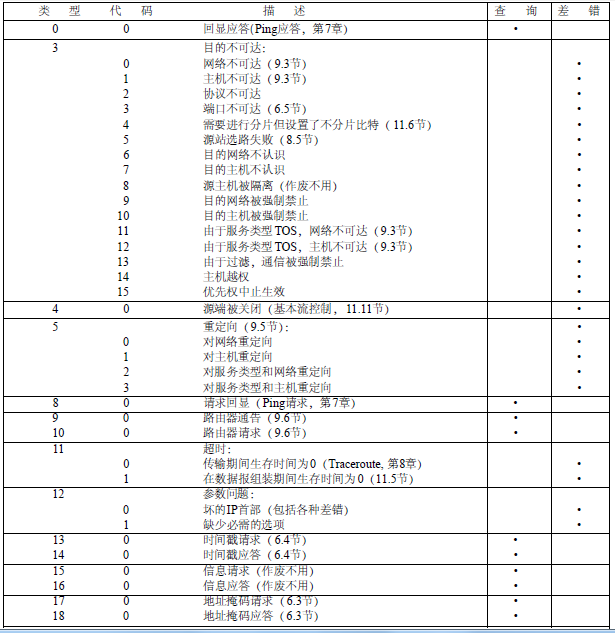
\includegraphics[width=0.4\textwidth]{icmp-message-type.png}
\caption{ICMP 类型}
\end{figure}

\subsection{Internet Group Management Protocol}
组播/多播. Class D 类 IP 地址. 
\begin{enumerate}
  \item 主机加入 multicast 组, 向该组的组播地址发送一个IGMP报文
  \item \textbf{本地组播路由器}收到IGMP报文后, 利用组播路由选择协议把这组成员关系发给因特网上的其他\textbf{组播路由器}
  \item \textbf{本地组播路由器}周期性探寻本地局域网上的主机, 以便知道这些主机是否还是组播组的成员. 
  \item 若几次探寻之后没有一个主机相应, 组播路由器认定本网络没有此组播组的主机, 不再把这组的成员关系发给其他的组播路由器
\end{enumerate}
\section{TCP/IP Routing Protocols (Gateway Protocols)}
Autonomous system (AS) 按区域划分的系统。每个AS由一组在相同管理者控制下的路由器组成。同一个AS内的路由器可运行相同的选路算法,且拥有相互之间的信息。

\begin{itemize}
  \item IGP (Interior Gateway Protocol) AS内使用
  \subitem RIP (Routing Information Protocol) 基于距离向量的路由协议。
  \subitem OSPF (Open Shortest Path First) Dijkstra最短费用路径算法,是一种链路状态协议。
  \item EGP (Exterior Gateway Protocol) 在各AS之间进行选路的选路算法。将分组从一个AS选路到另一个AS。
  \subitem BGP (Border Gateway Protocol)
\end{itemize}

\chapter{Data Link}
数据链路层. 
\section{Introduction}
信道类型
\begin{itemize}
  \item 一对一--点对点信道 (用户与ISP) 
  \item 一对多--广播信道 (总线型)
\end{itemize}
解决的问题
\begin{itemize}
  \item 封装成帧
  \item 透明传输 
  \item 差错检测 (CRC) 错了, 直接丢弃
\end{itemize}

\section{Cyclic Redundancy Check}
\begin{itemize}
  \item 以太网提供的服务是不可靠的交付,即尽最大努力的交付。
  \item 仅用循环冗余检验 CRC 差错检测技术只能做到无差错接受(accept)。
  \item “无差错接受”是指:“凡是接受的帧(即不包括丢弃的帧),我们都认为这些帧在传输过程中没有产生差错”。
  \item “凡是接收端数据链路层接受的帧都没有传输差错”(有差错的帧就丢弃而不接受)。
  \item 要做到“可靠传输”(即发送什么就收到什么)就必须再加上确认和重传机制。  
\end{itemize}
\subsection{Generation Algorithm}
\href{https://www.youtube.com/watch?v=6gbkoFciryA}{Error Detection and Correction 2: Cyclic Redundancy Check}

你得有一个生成多项式, 假设是 \texttt{1001 1}, 有一串数据, 假设是 \texttt{1101 0110 11}. 发送者和接收者必须得规定好相同的生成多项式. 在 IEEE 802.3 中规定的是 32 bit \texttt{0x82608EDB}. 
\begin{itemize}
  \item 弄明白生成多项式的阶. 
  \subitem 如果给你一串二进制数, 假设二进制数的长度为$r$ (当然前导0得去掉), 阶数就是$r-1$
  \subitem 因为$x^{r-1}+x^{r-2}+\dots+x^{1}+x^0$ MSB 表示的是 0 
  \item 在要发送的数据后面加上 $r$ 个0 (生成多项式的阶)
  \subitem 也就是 1101 0110 11\texttt{00 00} 记住是生成多项式的长度\textbf{减一}
  \item 拿\textbf{要发送的数据}模二除生成多项式
  \subitem Modulo 2\footnote{XOR} Division
\end{itemize}
\subsection{Modulo 2}
\begin{figure}[H]
\centering
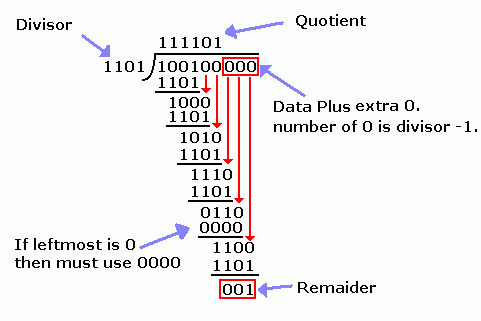
\includegraphics[width=0.33\textwidth]{crc_gen.png}
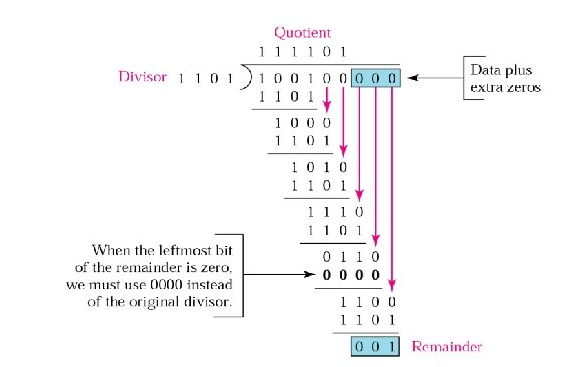
\includegraphics[width=0.33\textwidth]{crc_gen_3.png}
\caption{CRC 生成器}
\end{figure}

\begin{figure}[htbp]
\centering
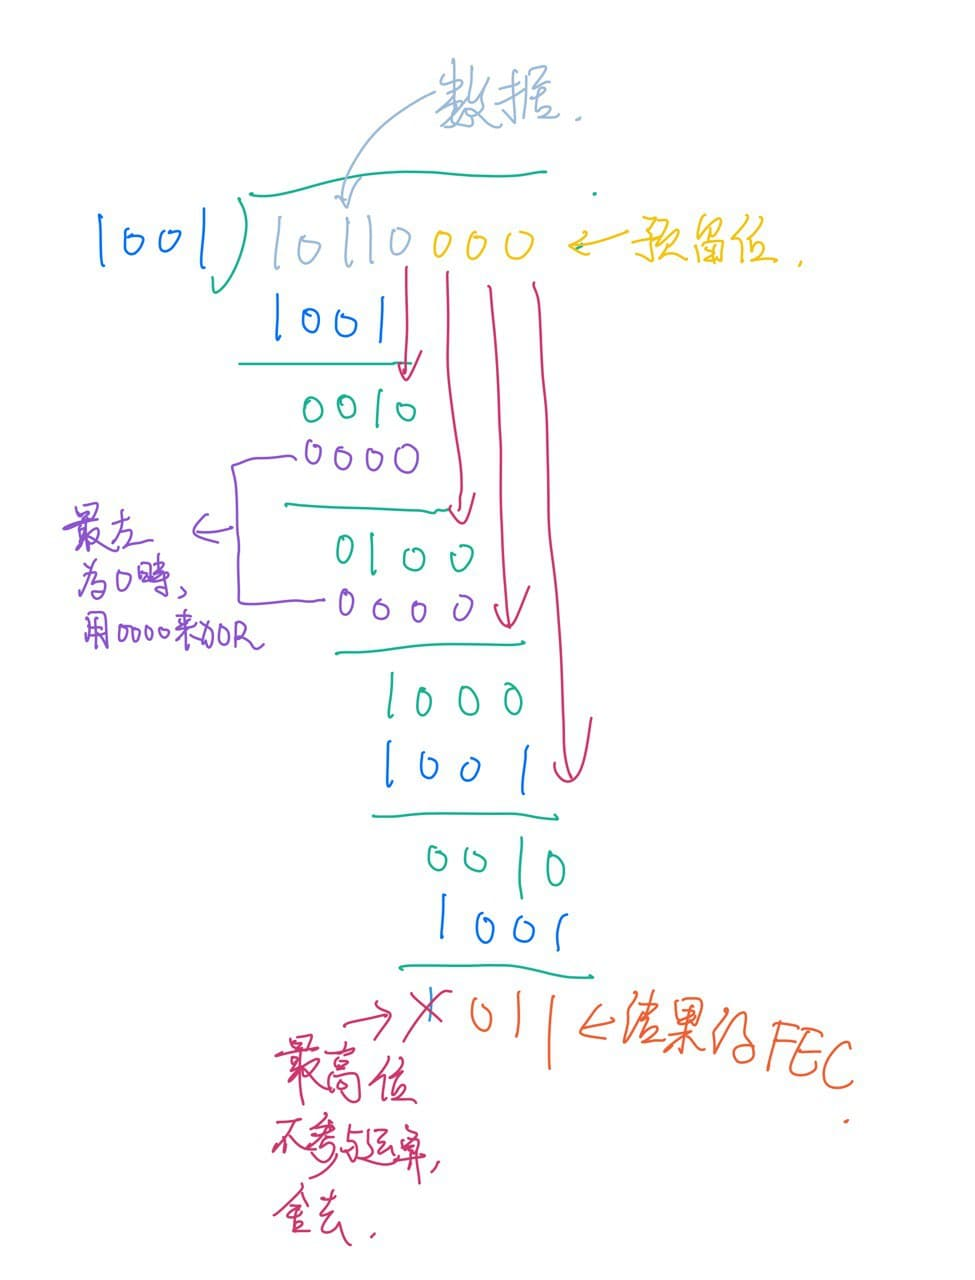
\includegraphics[width=0.5\textwidth]{crc_exp.jpg}
\caption{10110为数据, 1001为生成多项式}
\end{figure}
这些运算其实和除法没有任何关系, 只是借用了列竖式的形式计算而已. 

除数和被除数的MSB(左边)对齐, 写除数的那条横线, 长度和除数一样. 进行模二加之后往下走, \textbf{同时从原来的被除数上面补数下来}. 直到无数可补. 

每次最左边都要被舍弃掉的, 像个梯子一样往右移. 商在这里是没有意义的. 

如果XOR之后的结果最左边为0, 那么就先用0000来XOR (向右移动一位)

无数可补时的余数为FEC. 其长度就是刚开始补零的长度, 也就是生成多项式的二进制表示长度减一

把FEC换回刚开始补零的元数据出, 发出去
\subsection{Check Algorithm}
\begin{figure}[H]
\centering
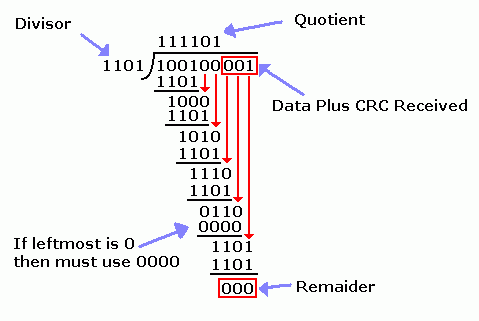
\includegraphics[width=0.33\textwidth]{crc_chk.png}
\caption{CRC 校验}
\end{figure}
拿带FEC的数据模二除以生成多项式. 余数为0则正确, 不为0则出错. 


\section{透明传输}
当所传数据中的比特组合恰巧与某一控制信息完全一样时, 采取适当措施, 使得接收方不会认为这样的数据是某种控制信息. 

\begin{itemize}
  \item 字节填充法. 填充一个 ESC 字节. (转义字符) 面向字符. 
  \item 零比特填充法. 面向比特. 
\end{itemize}



\section{Point-to-Point Protocol}
用户与ISP通信时使用协议

% Table generated by Excel2LaTeX from sheet 'Sheet3'
\begin{table}[htbp]
  \centering
    \begin{tabularx}{\textwidth}{|c|c|X|}
      \hline
    Field Name & Size (bytes) & Description \\
    \hline
    Flag  & 1     & Flag: Indicates the start of a PPP frame. Always has the value “01111110” binary (0x7E hexadecimal, or 126 decimal). \\
    \hline
    Address & 1     & Address: In HDLC this is the address of the destination of the frame. But in PPP we are dealing with a direct link between two devices, so this field has no real meaning. It is thus always set to “11111111” (0xFF or 255 decimal), which is equivalent to a broadcast (it means “all stations”). \\
    \hline
    Control & 1     & Control: This field is used in HDLC for various control purposes, but in PPP it is set to “00000011” (3 decimal). \\
    \hline
    Protocol & 2     & Protocol: Identifies the protocol of the datagram encapsulated in the Information field of the frame. See below for more information on the Protocol field. \\
    \hline
    Information & Variable & Information: Zero or more bytes of payload that contains either data or control information, depending on the frame type. For regular PPP data frames the network-layer datagram is encapsulated here. For control frames, the control information fields are placed here instead. \\
    \hline
    Padding & Variable & Padding: In some cases, additional dummy bytes may be added to pad out the size of the PPP frame. \\
    \hline
    FCS   & 2 (or 4) & Frame Check Sequence (FCS): A checksum computed over the frame to provide basic protection against errors in transmission. This is a CRC code similar to the one used for other layer two protocol error protection schemes such as the one used in Ethernet. It can be either 16 bits or 32 bits in size (default is 16 bits). \newline The FCS is calculated over the Address, Control, Protocol, Information and Padding fields. \\
    \hline
    Flag  & 1     & Flag: Indicates the end of a PPP frame. Always has the value “01111110” binary (0x7E hexadecimal, or 126 decimal). \\
    \hline
    \end{tabularx}%
  \caption{ PPP General Frame Format}
\end{table}%


\begin{figure}[H]
\centering
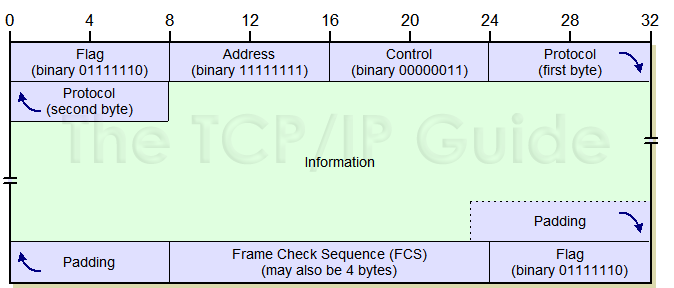
\includegraphics[width=0.8\textwidth]{pppformat.png}
\caption{PPP General Frame Format}
\end{figure}

\begin{itemize}
  \item header flag: 0x7e
  \item address: 0xff
  \item control: 0x03
  \item footer flag: 0x7e
\end{itemize}

\begin{itemize}
  \item 分组成帧
  \subitem PPP协议链路层的发送方必须能够携带网络层的分组,并将它封装在PPP链路层帧中,以便接收方能够确认链路层帧的起始和结束位置和该帧中网络层分组
  \item 透明性
  \subitem PPP协议不能对出现在网络层分组中的数据(首部或者数据)做任何限制。'
  \item 多种类型链路
  \subitem 除了要支持多种网络层的协议,PPP还必须能够在多种类型的链路上运行。\textbf{如:串行、并行、同步、异步、低速、高速等网络}
\end{itemize}

\section{Ethernet Frame}
\subsection{Media Access Control address}
48 bit (6 Bytes); 前3 Byte由IEEE规定(厂商编号), 后3 Byte由厂商自行规定. 
\paragraph{MAC广播地址}
全1地址。如以太网和令牌传递LAN,其广播地址是48个连续的1组成的字符串 FF-FF-FF-FF-FF-FF. 
\subsection{Frame}
An Ethernet packet starts with a seven-octet preamble and one-octet start frame delimiter (SFD).

% The preamble consists of a 56-bit (seven-byte) pattern of alternating 1 and 0 bits, allowing devices on the network to easily synchronize their receiver clocks, providing bit-level synchronization. It is followed by the SFD to provide byte-level synchronization and to mark a new incoming frame. 

Ethernet Frame 的MTU\footnote{maximum transmission unit. MTU应用于OSI模型的第二层数据链接层. 故IP MTU=Ethernet MTU=1500 Bytes. 也就是说MTU特指Ethernet Frame的载荷部分. }是1500 Bytes.\footnote{MTU 指的是其封装的数据帧, 总的最大是 1518 Bytes. (加上14 Bytes的首部和尾部 4 Bytes 的CRC/FEC) } 最小载荷长度为46 Bytes. 若不足则补零. 

the MTU for Ethernet is typically 1500 bytes. (The maximum packet length for Ethernet is typically 1518 bytes, but that includes 14 bytes of Ethernet header and 4 bytes of CRC, leaving 1500 bytes of payload).

\begin{figure}[H]
\centering
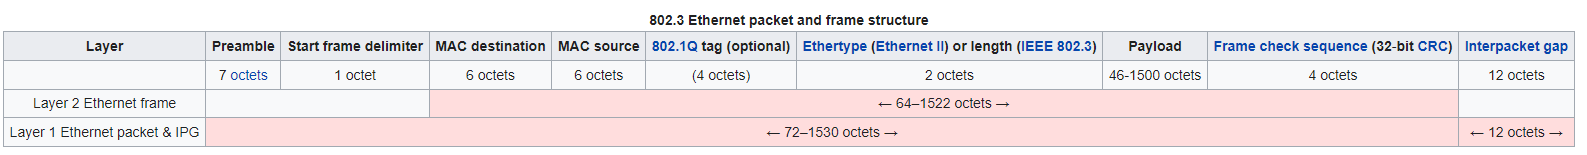
\includegraphics[width=\textwidth]{ethernet_frame_3.png}
\caption{802.3 Ethernet packet and frame structure}
\end{figure}

\begin{figure}[H]
\centering
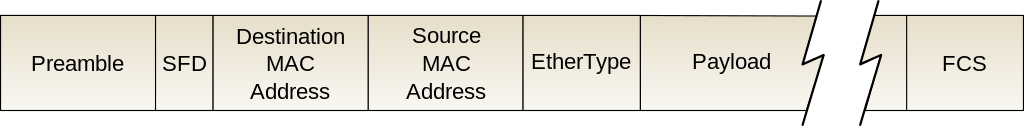
\includegraphics[width=0.8\textwidth]{ethernet_frame_2.png}
\caption{带有Preamble和SFD的以太网帧}
\end{figure}

\begin{figure}[H]
\centering
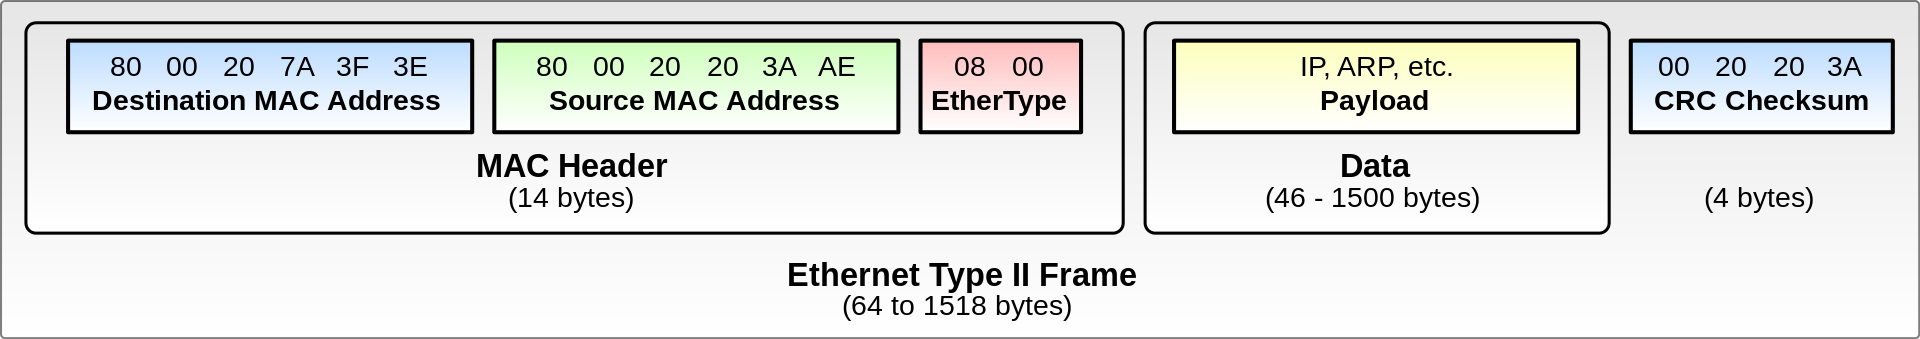
\includegraphics[width=0.8\textwidth]{ethernet_frame.png}
\caption{以太网帧}
\end{figure}



\begin{itemize}
  \item 以太网提供的服务是不可靠的交付,即尽最大努力的交付。
  \item 采用较为灵活的无连接的工作方式,即不必先建立连接就可以直接发送数据。 
  \item 以太网对发送的数据帧不进行编号,也不要求对方发回确认。
  \subitem 这样做的理由是局域网信道的质量很好,因信道质量产生差错的概率是很小的。 
\end{itemize}


\section{CSMA/CD}
Carrier Sense Multiple Access with Collision Detection. 信道并非在用户通信时固定分配给用户. 

\begin{itemize}
  \item CS 载波监听, 每一站在发送数据之前/之时都会检测总线上是否有其他计算机在发送数据
  \item MA 多点接入 (总线型网络)
  \item CD 边发送边监听 (半双工网络)
\end{itemize}

\begin{figure}[H]
\centering
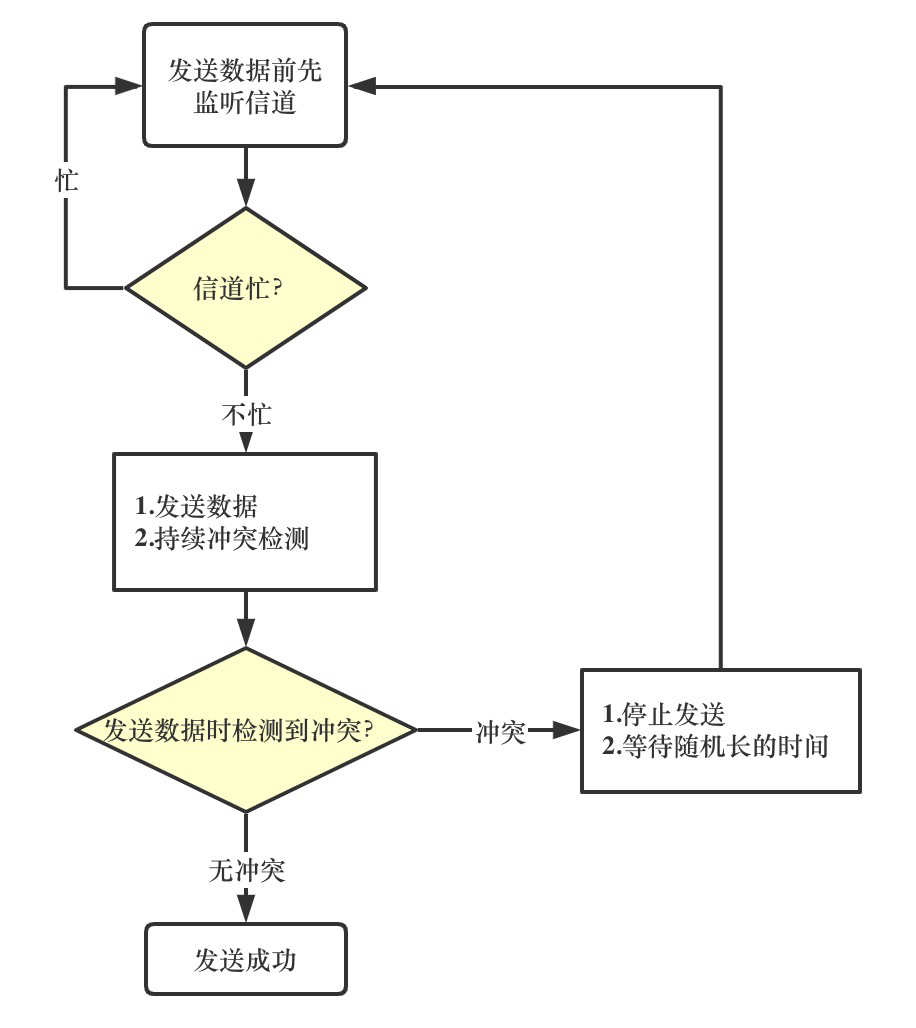
\includegraphics[width=0.5\textwidth]{csma_cd.png}
\caption{CSMA/CD}
\end{figure}

\begin{itemize}
  \item 先听后说,边听边说;
  \item 一旦冲突,立即停说;
  \item 等待时机,然后再说;
  \subitem 注:“听”,即监听、检测之意;“说”,即发送数据之意。
\end{itemize}


% \begin{enumerate}
%   \item 发送特殊阻塞信息并立即停止发送数据:特殊阻塞信息是连续几个字节的全1信号,此举意在强化碰撞,以使得其它设备能尽快检测到碰撞发生。
%   \item 在固定时间(一开始是1 contention period times)内等待随机的时间,再次发送。
%   \item 若依旧碰撞,则采用截断二进制指数避退算法进行发送。即十次之内停止前一次“固定时间”的两倍时间内随机再发送,十次后则停止前一次“固定时间”内随机再发送。尝试16次之后仍然失败则放弃发送。
% \end{enumerate}

\subsection{二进制指数类型退避算法}
truncated binary exponential type

发生碰撞的站在停止发送数据后,要推迟(退避)一个随机时间才能再发送数据。
\begin{itemize}
  \item 基本退避时间取为争用期 2$\tau$
  \item 从整数集合[0,1,\dots, $2k -1$]中随机地取出一个数,记为 $r$。重传所需的时延就是 $r$ 倍的基本退避时间。
  \subitem 参数 $k$ 按下面的公式计算:$k = \min$[重传次数, 10]
  \subitem 当 $k \leq 10$ 时,参数 $k$ 等于重传次数。
  \subitem 在第一次重传时,$k=1$,随机数$r$从整数$\{0,1\}$中选一个数,可得重传的推迟时间要么为0,要么为$r\times 2\tau=1\times 2\tau$, 这两个选择一个。
  \subitem 如果再次发送,即第二次重传,$k=2$,代入[0,1,2,3\dots,$2^{k-1}$] ,随机数$r$从整数$\{0,1,2,3\}$选一个数,可得重传推迟时间是0,2$\tau$,4$\tau$,6$\tau$ 这4个值随机选择一个。
  \subitem 当$k=3$时,$r=\{0,1,2,3,4,5,6,7\}$ 以此类推. 
  \subitem 当$k>10$时,$k = \min$[重传次数, 10]
  \item 当重传达 16 次仍不能成功时即丢弃该帧(表明同时打算发送数据的站太多,以至连续发生冲突),并向高层报告。 
\end{itemize}

使用上述退避算法可使得重传的平均时间重传次数而增大,因而减少发生碰撞的概率,有利于系统的稳定。

\section{Bridge}
\begin{figure}[H]
\centering
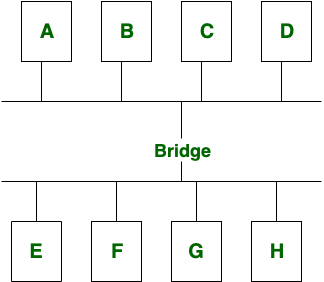
\includegraphics[width=0.33\textwidth]{bridge.png}
\caption{Bridge}
\end{figure}

% Table generated by Excel2LaTeX from sheet 'Sheet1'
\begin{table}[htbp]
  \centering
    \begin{tabularx}{\textwidth}{XX}
      \hline
    \textbf{Hub} & \textbf{Bridge} \\
    \hline
    Hub is network device which is used for connecting number of devices.\newline 用来连接多个设备  & Bridge is also a network device which is used to connect two different LAN working on same protocol. \newline 用来连接使用同一协议的不同的 LAN \\
    \hdashline
    Types of Hub are: Active and Passive. & Types of bridge are: Source route, Transparent and Translation. \\
    \hdashline
    Hub does not perform data filtration. & While bridge performs data filtration. \newline 网桥会进行数据过滤 \\
    \hdashline
    There are multiple ports are used in Hub. \newline 集线器有多个端口 & But in bridge one port for incoming and another port for outgoing. \newline 网桥只有一入一出 \\
    \hdashline
    Hub connects the LAN`s segment. & While bridge connects two different LAN working on same protocol. \newline 网桥连接两个工作在同一协议的局域网\\
    \hdashline
    Hub operates on the physical layer of the ISO-OSI Model. & While bridge operates on the data link layer of the ISO-OSI model. \newline 物理层和数据链路层 \\
    \hline
    \end{tabularx}%
  \caption{网桥和集线器区别}
\end{table}%


\section{Switch}
在集线器的基础上,添加了MAC地址学习功能,成为了交换机,这样可以避免集线器对所有帧都广播的弊病。

交换机在数据通信中完成两个基本的操作. 
\begin{itemize}
  \item 构造和维护 MAC 地址表
  \item 交换数据帧
  \subitem 打开源端口与目标端口之间的数据通道,把数据帧转发到目标端口上。 
\end{itemize}
可以用于隔离冲突域, 但是不能隔离广播域. 

\subsection{MAC 地址表}
在交换机中,有一个交换地址表(思科交换机中称为CAM 表),记录着主机 MAC 地址和该主机所连接的交换机端口号之间的对应关系,由交换机采用动态自学习的方法构造和维护。 

交换机在重新启动或手工清除MAC 地址表后,MAC 地址表没有任何MAC 地址的记录。 

\section{Address Resolution Protocol}
节点的三种不同地址表示

ARP is layer 2. The reason being is that a broadcast is sent on layer 2 (data link layer) and ARP will normally not traverse to layer 3 (network layer). However it can provide extra features to the layer 3 protocol.
\begin{itemize}
  \item 应用层的主机名
  \subitem DNS将主机名解析到IP地址。
  \item 网络层的IP地址
  \subitem ARP将IP地址解析到MAC地址。
  \item 链路层的MAC地址
\end{itemize}
ARP只为在同一个LAN上的节点解析IP地址。实际在链路上传输时,根据MAC地址,确定相应的节点. 
\section{Virtual Local Area Network}
\subsection{Flooding}
主机A向主机B通信,它首先广播一个ARP请求,以获取主机B的MAC地址。此时主机A上连的二层交换机收到ARP广播后,会将它转发给除接收端口外的其他所有端口,也就是洪泛(Flooding)。
\begin{itemize}
  \item 在交换机构成的网络中,所有设备都会转发广播帧,因此任何一个广播帧或多播帧都将被广播到整个局域网中的每一台主机。
  \item 其他的收到这个广播帧的交换机(包括三层交换机)也会作同样的处理,最终ARP 请求会被转发到同一网络中的所有主机上。
  \item 如果此时网络中的其他主机也要和别的主机进行通信,必然产生大量的广播。
\end{itemize}
在网络通信中,广播信息是普遍存在的,这些广播帧将占用大量的网络带宽,导致网络速度和通信效率的下降,并额外增加了网络主机为处理广播信息所产生的负荷。 
\subsection{VLAN}
路由器能实现对广播域的分割和隔离, 但路由器所带的以太网接口数量很少,一般为1$\sim$4 个,远远不能满足对网络分段的需要,而交换机配备有较多的以太网端口,\textbf{为在交换机中实现不同网段的广播隔离产生了VLAN 交换技术。 }
\begin{itemize}
  \item 在交换机上划分VLAN,一个VLAN 就是一个网段
  \item 同一交换机上可划分不同的VLAN,不同的交换机上可属于同一个VLAN
  \item 可将一个大的局域网划分成若干个网段,每个网段内所有主机间的通信和广播仅限于该VLAN 内,广播帧不会被转发到其他网段。
  \item 一个VLAN 就是一个广播域,VLAN 间不能直接通信,从而实现了对广播域的分割和隔离
\end{itemize}
\section{Dynamic Host Configuration Protocol}
自动给终端设备分配IP地址,子网掩码,默认网关和DNS服务器的地址,同时也可以给终端设备自动匹配其他选项. 使用UDP(67,68)端口. DHCP必须知道
\begin{itemize}
  \item 客户端设备所在网络的子网掩码
  \subitem DHCP服务器依据子网掩码的信息来判断,服务器该分配哪个IP地址,以使该IP地址在那个子网内
  \item 客户端的MAC地址
\end{itemize}

\chapter{Physical}
100Base-T 双绞线 (Twisted-pairs)

\section{Hub}
A Hub is a layer-1 device and operates only in the physical network of the OSI Model. 

\begin{figure}[H]
\centering
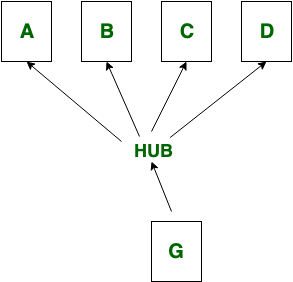
\includegraphics[width=0.33\textwidth]{hub.png}
\caption{集线器}
\end{figure}

中继器(一入一出), 集线器(一入多出)用于再生, 放大信号

ADSL 双绞线(原电话线进行改造) 

光纤同轴混合网 (光纤, 转接同轴电缆) (有线电视网改造)
\chapter{Security}
\begin{itemize}
  \item 被动攻击
  \subitem 截获
  \subitem 篡改
  \item 主动攻击
  \subitem 恶意程序
  \subitem DoS
\end{itemize}

\begin{itemize}
  \item 对称密钥体制 
  \subitem  Data Encryption Standard
  \item 公钥密码体制 
  \subitem Digital Signature Algorithm (DSA​)
  \subitem Rivest-Shamir-Adleman (RSA) algorithm
\end{itemize}

\section{Protocols}
\subsection{Transport Layer Security}
运输层安全协议

传输层安全性协议(英语:Transport Layer Security,缩写:TLS)及其前身安全套接层(英语:Secure Sockets Layer,缩写:SSL)是一种安全协议,目的是为互联网通信提供安全及数据完整性保障。
\subsection{Pretty Good Privacy}
应用层的安全协议

PGP(英语:Pretty Good Privacy,直译:优良保密协议)是一套用于讯息加密、验证的应用程序。
\section{Intrusion Detection System}


\end{document}






% Table generated by Excel2LaTeX from sheet 'Sheet2'
    % \begin{tabularx}{\textwidth}{ccccc}
% \begin{longtable}{ccccc}
%   \label{tab:ip_protocol}%
%   \caption{RFC 790}
%     % \begin{tabularx}{\textwidth}{XXXXX}
%       \endfirsthead
    
%     % \hline
%     Hex   & Protocol Number & Keyword & Protocol & References/RFC \\
%     % \hline
%     \endhead

%     % \hline
%     \endfoot

%     0x00  & 0     & HOPOPT & IPv6 Hop-by-Hop Option & RFC 8200 \\
%     0x01  & 1     & ICMP  & Internet Control Message Protocol & RFC 792 \\
%     0x02  & 2     & IGMP  & Internet Group Management Protocol & RFC 1112 \\
%     0x03  & 3     & GGP   & Gateway-to-Gateway Protocol & RFC 823 \\
%     0x04  & 4     & IP-in-IP & IP in IP (encapsulation) & RFC 2003 \\
%     0x05  & 5     & ST    & Internet Stream Protocol & RFC 1190, RFC 1819 \\
%     0x06  & 6     & TCP   & Transmission Control Protocol & RFC 793 \\
%     0x07  & 7     & CBT   & Core-based trees & RFC 2189 \\
%     0x08  & 8     & EGP   & Exterior Gateway Protocol & RFC 888 \\
%     0x09  & 9     & IGP   & Interior Gateway Protocol (any private interior gateway, for example Cisco's IGRP) &  \\
%     0x0A  & 10    & BBN-RCC-MON & BBN RCC Monitoring &  \\
%     0x0B  & 11    & NVP-II & Network Voice Protocol & RFC 741 \\
%     0x0C  & 12    & PUP   & Xerox PUP &  \\
%     0x0D  & 13    & ARGUS & ARGUS &  \\
%     0x0E  & 14    & EMCON & EMCON &  \\
%     0x0F  & 15    & XNET  & Cross Net Debugger & IEN 158[2] \\
%     0x10  & 16    & CHAOS & Chaos &  \\
%     0x11  & 17    & UDP   & User Datagram Protocol & RFC 768 \\
%     0x12  & 18    & MUX   & Multiplexing & IEN 90[3] \\
%     0x13  & 19    & DCN-MEAS & DCN Measurement Subsystems &  \\
%     0x14  & 20    & HMP   & Host Monitoring Protocol & RFC 869 \\
%     0x15  & 21    & PRM   & Packet Radio Measurement &  \\
%     0x16  & 22    & XNS-IDP & XEROX NS IDP &  \\
%     0x17  & 23    & TRUNK-1 & Trunk-1 &  \\
%     0x18  & 24    & TRUNK-2 & Trunk-2 &  \\
%     0x19  & 25    & LEAF-1 & Leaf-1 &  \\
%     0x1A  & 26    & LEAF-2 & Leaf-2 &  \\
%     0x1B  & 27    & RDP   & Reliable Data Protocol & RFC 908 \\
%     0x1C  & 28    & IRTP  & Internet Reliable Transaction Protocol & RFC 938 \\
%     0x1D  & 29    & ISO-TP4 & ISO Transport Protocol Class 4 & RFC 905 \\
%     0x1E  & 30    & NETBLT & Bulk Data Transfer Protocol & RFC 998 \\
%     0x1F  & 31    & MFE-NSP & MFE Network Services Protocol &  \\
%     0x20  & 32    & MERIT-INP & MERIT Internodal Protocol &  \\
%     0x21  & 33    & DCCP  & Datagram Congestion Control Protocol & RFC 4340 \\
%     0x22  & 34    & 3PC   & Third Party Connect Protocol &  \\
%     0x23  & 35    & IDPR  & Inter-Domain Policy Routing Protocol & RFC 1479 \\
%     0x24  & 36    & XTP   & Xpress Transport Protocol &  \\
%     0x25  & 37    & DDP   & Datagram Delivery Protocol &  \\
%     0x26  & 38    & IDPR-CMTP & IDPR Control Message Transport Protocol &  \\
%     0x27  & 39    & TP++  & TP++ Transport Protocol &  \\
%     0x28  & 40    & IL    & IL Transport Protocol &  \\
%     0x29  & 41    & IPv6  & IPv6 Encapsulation & RFC 2473 \\
%     0x2A  & 42    & SDRP  & Source Demand Routing Protocol & RFC 1940 \\
%     0x2B  & 43    & IPv6-Route & Routing Header for IPv6 & RFC 8200 \\
%     0x2C  & 44    & IPv6-Frag & Fragment Header for IPv6 & RFC 8200 \\
%     0x2D  & 45    & IDRP  & Inter-Domain Routing Protocol &  \\
%     0x2E  & 46    & RSVP  & Resource Reservation Protocol & RFC 2205 \\
%     0x2F  & 47    & GRE   & Generic Routing Encapsulation & RFC 2784, RFC 2890 \\
%     0x30  & 48    & DSR   & Dynamic Source Routing Protocol & RFC 4728 \\
%     0x31  & 49    & BNA   & Burroughs Network Architecture &  \\
%     0x32  & 50    & ESP   & Encapsulating Security Payload & RFC 4303 \\
%     0x33  & 51    & AH    & Authentication Header & RFC 4302 \\
%     0x34  & 52    & I-NLSP & Integrated Net Layer Security Protocol & TUBA \\
%     0x35  & 53    & SwIPe & SwIPe & RFC 5237 \\
%     0x36  & 54    & NARP  & NBMA Address Resolution Protocol & RFC 1735 \\
%     0x37  & 55    & MOBILE & IP Mobility (Min Encap) & RFC 2004 \\
%     0x38  & 56    & TLSP  & Transport Layer Security Protocol (using Kryptonet key management) &  \\
%     0x39  & 57    & SKIP  & Simple Key-Management for Internet Protocol & RFC 2356 \\
%     0x3A  & 58    & IPv6-ICMP & ICMP for IPv6 & RFC 4443, RFC 4884 \\
%     0x3B  & 59    & IPv6-NoNxt & No Next Header for IPv6 & RFC 8200 \\
%     0x3C  & 60    & IPv6-Opts & Destination Options for IPv6 & RFC 8200 \\
%     0x3D  & 61    &       & Any host internal protocol &  \\
%     0x3E  & 62    & CFTP  & CFTP  &  \\
%     0x3F  & 63    &       & Any local network &  \\
%     0x40  & 64    & SAT-EXPAK & SATNET and Backroom EXPAK &  \\
%     0x41  & 65    & KRYPTOLAN & Kryptolan &  \\
%     0x42  & 66    & RVD   & MIT Remote Virtual Disk Protocol &  \\
%     0x43  & 67    & IPPC  & Internet Pluribus Packet Core &  \\
%     0x44  & 68    &       & Any distributed file system &  \\
%     0x45  & 69    & SAT-MON & SATNET Monitoring &  \\
%     0x46  & 70    & VISA  & VISA Protocol &  \\
%     0x47  & 71    & IPCU  & Internet Packet Core Utility &  \\
%     0x48  & 72    & CPNX  & Computer Protocol Network Executive &  \\
%     0x49  & 73    & CPHB  & Computer Protocol Heart Beat &  \\
%     0x4A  & 74    & WSN   & Wang Span Network &  \\
%     0x4B  & 75    & PVP   & Packet Video Protocol &  \\
%     0x4C  & 76    & BR-SAT-MON & Backroom SATNET Monitoring &  \\
%     0x4D  & 77    & SUN-ND & SUN ND PROTOCOL-Temporary &  \\
%     0x4E  & 78    & WB-MON & WIDEBAND Monitoring &  \\
%     0x4F  & 79    & WB-EXPAK & WIDEBAND EXPAK &  \\
%     0x50  & 80    & ISO-IP & International Organization for Standardization Internet Protocol &  \\
%     0x51  & 81    & VMTP  & Versatile Message Transaction Protocol & RFC 1045 \\
%     0x52  & 82    & SECURE-VMTP & Secure Versatile Message Transaction Protocol & RFC 1045 \\
%     0x53  & 83    & VINES & VINES &  \\
%     0x54  & 84    & TTP   & TTP   &  \\
%     0x54  & 84    & IPTM  & Internet Protocol Traffic Manager &  \\
%     0x55  & 85    & NSFNET-IGP & NSFNET-IGP &  \\
%     0x56  & 86    & DGP   & Dissimilar Gateway Protocol &  \\
%     0x57  & 87    & TCF   & TCF   &  \\
%     0x58  & 88    & EIGRP & EIGRP & Informational RFC 7868 \\
%     0x59  & 89    & OSPF  & Open Shortest Path First & RFC 2328 \\
%     0x5A  & 90    & Sprite-RPC & Sprite RPC Protocol &  \\
%     0x5B  & 91    & LARP  & Locus Address Resolution Protocol &  \\
%     0x5C  & 92    & MTP   & Multicast Transport Protocol &  \\
%     0x5D  & 93    & AX.25 & AX.25 &  \\
%     0x5E  & 94    & OS    & KA9Q NOS compatible IP over IP tunneling &  \\
%     0x5F  & 95    & MICP  & Mobile Internetworking Control Protocol &  \\
%     0x60  & 96    & SCC-SP & Semaphore Communications Sec. Pro &  \\
%     0x61  & 97    & ETHERIP & Ethernet-within-IP Encapsulation & RFC 3378 \\
%     0x62  & 98    & ENCAP & Encapsulation Header & RFC 1241 \\
%     0x63  & 99    &       & Any private encryption scheme &  \\
%     0x64  & 100   & GMTP  & GMTP  &  \\
%     0x65  & 101   & IFMP  & Ipsilon Flow Management Protocol &  \\
%     0x66  & 102   & PNNI  & PNNI over IP &  \\
%     0x67  & 103   & PIM   & Protocol Independent Multicast &  \\
%     0x68  & 104   & ARIS  & IBM's ARIS (Aggregate Route IP Switching) Protocol &  \\
%     0x69  & 105   & SCPS  & SCPS (Space Communications Protocol Standards) & SCPS-TP[4] \\
%     0x6A  & 106   & QNX   & QNX   &  \\
%     0x6B  & 107   & A/N   & Active Networks &  \\
%     0x6C  & 108   & IPComp & IP Payload Compression Protocol & RFC 3173 \\
%     0x6D  & 109   & SNP   & Sitara Networks Protocol &  \\
%     0x6E  & 110   & Compaq-Peer & Compaq Peer Protocol &  \\
%     0x6F  & 111   & IPX-in-IP & IPX in IP &  \\
%     0x70  & 112   & VRRP  & Virtual Router Redundancy Protocol, Common Address Redundancy Protocol (not IANA assigned) & VRRP:RFC 3768 \\
%     0x71  & 113   & PGM   & PGM Reliable Transport Protocol & RFC 3208 \\
%     0x72  & 114   &       & Any 0-hop protocol &  \\
%     0x73  & 115   & L2TP  & Layer Two Tunneling Protocol Version 3 & RFC 3931 \\
%     0x74  & 116   & DDX   & D-II Data Exchange (DDX) &  \\
%     0x75  & 117   & IATP  & Interactive Agent Transfer Protocol &  \\
%     0x76  & 118   & STP   & Schedule Transfer Protocol &  \\
%     0x77  & 119   & SRP   & SpectraLink Radio Protocol &  \\
%     0x78  & 120   & UTI   & Universal Transport Interface Protocol &  \\
%     0x79  & 121   & SMP   & Simple Message Protocol &  \\
%     0x7A  & 122   & SM    & Simple Multicast Protocol & draft-perlman-simple-multicast-03 \\
%     0x7B  & 123   & PTP   & Performance Transparency Protocol &  \\
%     0x7C  & 124   & IS-IS over IPv4 & Intermediate System to Intermediate System (IS-IS) Protocol over IPv4 & RFC 1142 and RFC 1195 \\
%     0x7D  & 125   & FIRE  & Flexible Intra-AS Routing Environment &  \\
%     0x7E  & 126   & CRTP  & Combat Radio Transport Protocol &  \\
%     0x7F  & 127   & CRUDP & Combat Radio User Datagram &  \\
%     0x80  & 128   & SSCOPMCE & Service-Specific Connection-Oriented Protocol in a Multilink and Connectionless Environment & ITU-T Q.2111 (1999) \\
%     0x81  & 129   & IPLT  &       &  \\
%     0x82  & 130   & SPS   & Secure Packet Shield &  \\
%     0x83  & 131   & PIPE  & Private IP Encapsulation within IP & Expired I-D draft-petri-mobileip-pipe-00.txt \\
%     0x84  & 132   & SCTP  & Stream Control Transmission Protocol & RFC 4960 \\
%     0x85  & 133   & FC    & Fibre Channel &  \\
%     0x86  & 134   & RSVP-E2E-IGNORE & Reservation Protocol (RSVP) End-to-End Ignore & RFC 3175 \\
%     0x87  & 135   & Mobility Header & Mobility Extension Header for IPv6 & RFC 6275 \\
%     0x88  & 136   & UDPLite & Lightweight User Datagram Protocol & RFC 3828 \\
%     0x89  & 137   & MPLS-in-IP & Multiprotocol Label Switching Encapsulated in IP & RFC 4023, RFC 5332 \\
%     0x8A  & 138   & manet & MANET Protocols & RFC 5498 \\
%     0x8B  & 139   & HIP   & Host Identity Protocol & RFC 5201 \\
%     0x8C  & 140   & Shim6 & Site Multihoming by IPv6 Intermediation & RFC 5533 \\
%     0x8D  & 141   & WESP  & Wrapped Encapsulating Security Payload & RFC 5840 \\
%     0x8E  & 142   & ROHC  & Robust Header Compression & RFC 5856 \\
%     0x8F  & 143   & Ethernet & IPv6 Segment Routing (TEMPORARY - registered 2020-01-31, expires 2021-01-31) &  \\
%     0x90-0xFC & 144-252 & Unassigned &       &  \\
%     0xFD-0xFE & 253-254 & Use for experimentation and testing &       & RFC 3692 \\
%     0xFF  & 255   & Reserved &       &  \\
% \end{longtable}%